\documentclass[../thesis.tex]{subfiles}
\begin{document}

\section{FSC-147}
FSC-147 \cite{ranjan2021Famnet} is a recent few-shot counting (FSC) dataset. It was introduced in 2021 and has since become the most widely used dataset in the field of class-agnostic counting.
This is due to its diverse range of images, which contain varied classes, compositions, and cameras.
The two most significant features of a class-agnostic counting dataset are (i) its ability to measure the accuracy of a method at finding the correct count and (ii) its ability to test how well a method generalises to previously unseen classes. 
The former requires an accurate knowledge of the number of objects in each image.
The latter is achieved by having complete mutual exclusivity between the classes seen during training, validation, and testing. 
FSC-147 includes 6135 images.
Each image has point annotations for each object instance and three random instance bounding box annotations, all of which were manually gathered. 
FSC-147 is a single-class dataset;  only one labelled type of object is present per image. 
While there are some examples which contain more than one kind of object, these are rare and only one class is labelled.

\subsection{Limitations}\label{sec__FSC133__limitations}
While FSC-147 has proven invaluable as a dataset for counting, the limited annotations do not allow for methods to develop a complex understanding of the task.
These limitations include the small number of bounding box annotations per image, the lack of pixel-wise segmentations of any objects, and no information on the occlusion of objects in an image.
The lack of information about instance occlusion can lead to methods struggling to gain a coherent understanding of counting in high-occlusion scenarios.
Most methods that use FSC-147 utilise a loss function based on a regressed density map prediction. 
Instead of their loss comparing the generated density map to a ground truth density map, they must compare to a pseudo-ground-truth density map which features a Gaussian kernel centred at each instance annotation. 
These Gaussian kernels lose a lot of the salient information about the objects they represent, like shape and scale, which is then lost to the method.
Methods also develop an inconsistent view of which objects should be counted when there is occlusion involved. 
This is due to the fact it is not possible to construct a set of rigorous rules about which objects are too occluded to be counted, meaning these decisions are made subjectively and therefore inconsistently.
This is made clear with the examples we present in \Cref{sec__FSC133__errors__countdiscrepancy}.

The single-class nature of this dataset means that methods trained on it are not incentivised to learn discriminative features. 
The tasks can often be solved by counting all objects present rather than focusing on whether the objects in the image are similar to each other or the exemplar. 
This leads to the methods becoming `generic object detectors' rather than counters which locate repeated instances of the same type.
The images are also relatively simple, with a clear class to count. This is made clear by our work in \Cref{sec__LTCA} which achieves state-of-the-art results on this dataset with no user input. 
The lack of multi-class and highly complex images 
limits the capacity of methods using this dataset to be developed or tested in many realistic settings where more than one kind of countable object could be present.


\subsection{Errors}
There are errors in FSC-147, including incorrect annotations and, more significantly, the repetition of images and the overlap between training, validation, and test sets. Some of these errors are presented in \Cref{fig__FSC133__subset_dupes}.
These errors undermine the judgements that can be made about the accuracy of a given method as well as a method's ability to generalise to unseen classes.


\begin{figure}
    \centering
    Train \\ \vspace{0.25em}
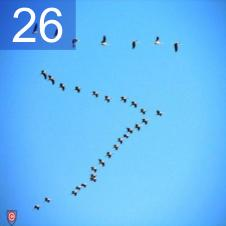
\includegraphics[height=0.15\textwidth, width=0.15\textwidth]{../files/appendicies/FSC133/images/numbered_ims/4399.jpg}%
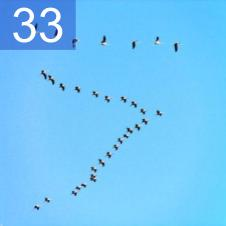
\includegraphics[height=0.15\textwidth, width=0.15\textwidth]{../files/appendicies/FSC133/images/numbered_ims/4620.jpg}%
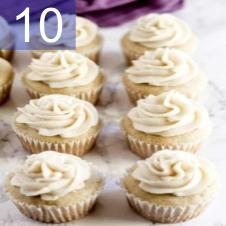
\includegraphics[height=0.15\textwidth, width=0.15\textwidth]{../files/appendicies/FSC133/images/numbered_ims/3812.jpg}%
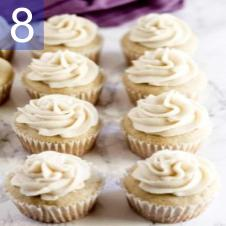
\includegraphics[height=0.15\textwidth, width=0.15\textwidth]{../files/appendicies/FSC133/images/numbered_ims/5238.jpg}%
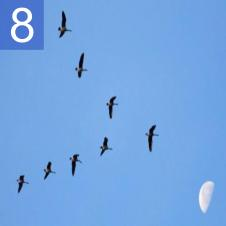
\includegraphics[height=0.15\textwidth, width=0.15\textwidth]{../files/appendicies/FSC133/images/numbered_ims/6684.jpg}%
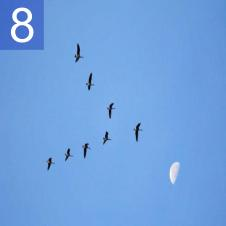
\includegraphics[height=0.15\textwidth,
width=0.15\textwidth]{../files/appendicies/FSC133/images/numbered_ims/4350.jpg}%
\\
\vspace{-0.5em}

\includegraphics[height=0.15\textwidth, width=0.15\textwidth]{../files/appendicies/FSC133/images/numbered_ims/3462.jpg}%

\includegraphics[height=0.15\textwidth, width=0.15\textwidth]{../files/appendicies/FSC133/images/numbered_ims/5638.jpg}%
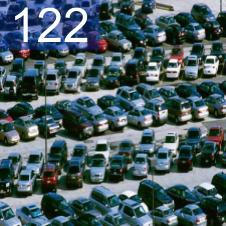
\includegraphics[height=0.15\textwidth, width=0.15\textwidth]{../files/appendicies/FSC133/images/numbered_ims/6138.jpg}%
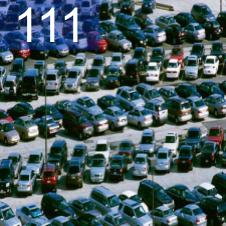
\includegraphics[height=0.15\textwidth, width=0.15\textwidth]{../files/appendicies/FSC133/images/numbered_ims/6864.jpg}%
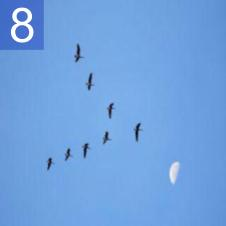
\includegraphics[height=0.15\textwidth, width=0.15\textwidth]{../files/appendicies/FSC133/images/numbered_ims/4707.jpg}%
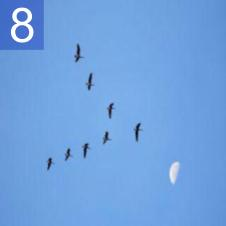
\includegraphics[height=0.15\textwidth, width=0.15\textwidth]{../files/appendicies/FSC133/images/numbered_ims/4683.jpg}%
\\
\vspace{-0.5em}

\includegraphics[height=0.15\textwidth, width=0.15\textwidth]{../files/appendicies/FSC133/images/numbered_ims/3506.jpg}%
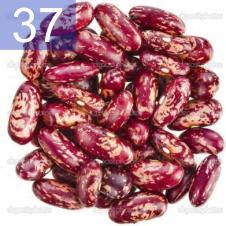
\includegraphics[height=0.15\textwidth, width=0.15\textwidth]{../files/appendicies/FSC133/images/numbered_ims/3791.jpg}%
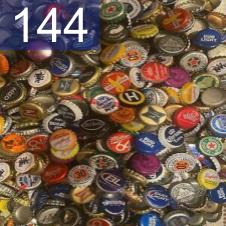
\includegraphics[height=0.15\textwidth, width=0.15\textwidth]{../files/appendicies/FSC133/images/numbered_ims/2891.jpg}%
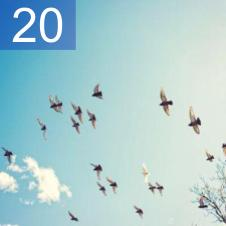
\includegraphics[height=0.15\textwidth, width=0.15\textwidth]{../files/appendicies/FSC133/images/numbered_ims/4386.jpg}%
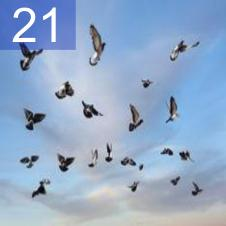
\includegraphics[height=0.15\textwidth, width=0.15\textwidth]{../files/appendicies/FSC133/images/numbered_ims/6567.jpg}%
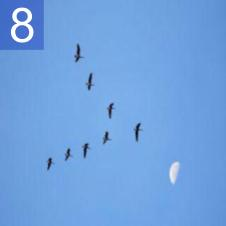
\includegraphics[height=0.15\textwidth, width=0.15\textwidth]{../files/appendicies/FSC133/images/numbered_ims/4375.jpg}%
\\
Val \\ \vspace{0.25em}
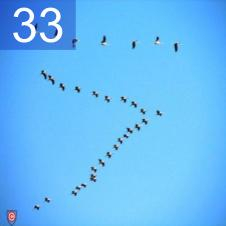
\includegraphics[height=0.15\textwidth, width=0.15\textwidth]{../files/appendicies/FSC133/images/numbered_ims/4549.jpg}%
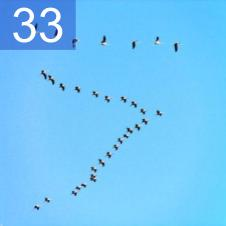
\includegraphics[height=0.15\textwidth, width=0.15\textwidth]{../files/appendicies/FSC133/images/numbered_ims/4719.jpg}%
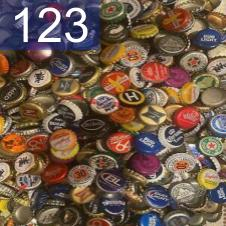
\includegraphics[height=0.15\textwidth, width=0.15\textwidth]{../files/appendicies/FSC133/images/numbered_ims/1896.jpg}%
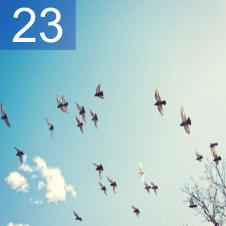
\includegraphics[height=0.15\textwidth, width=0.15\textwidth]{../files/appendicies/FSC133/images/numbered_ims/7415.jpg}%
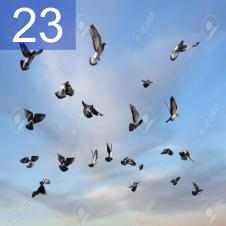
\includegraphics[height=0.15\textwidth, width=0.15\textwidth]{../files/appendicies/FSC133/images/numbered_ims/929.jpg}%
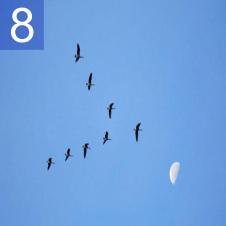
\includegraphics[height=0.15\textwidth, width=0.15\textwidth]{../files/appendicies/FSC133/images/numbered_ims/4704.jpg}%
\\
Test \\ \vspace{0.25em}

\includegraphics[height=0.15\textwidth, width=0.15\textwidth]{../files/appendicies/FSC133/images/numbered_ims/3698.jpg}%
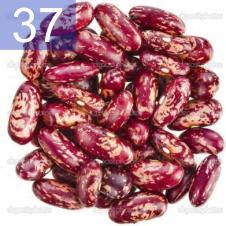
\includegraphics[height=0.15\textwidth, width=0.15\textwidth]{../files/appendicies/FSC133/images/numbered_ims/3494.jpg}%
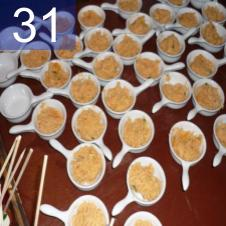
\includegraphics[height=0.15\textwidth, width=0.15\textwidth]{../files/appendicies/FSC133/images/numbered_ims/3282.jpg}%
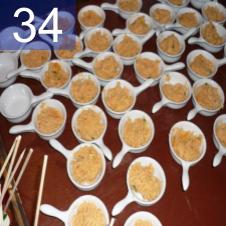
\includegraphics[height=0.15\textwidth, width=0.15\textwidth]{../files/appendicies/FSC133/images/numbered_ims/3285.jpg}%
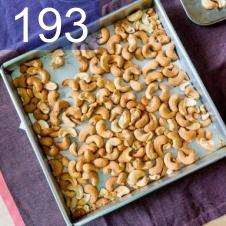
\includegraphics[height=0.15\textwidth, width=0.15\textwidth]{../files/appendicies/FSC133/images/numbered_ims/5142.jpg}%
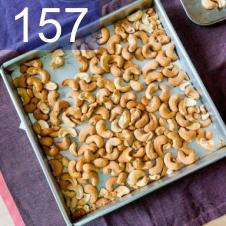
\includegraphics[height=0.15\textwidth, width=0.15\textwidth]{../files/appendicies/FSC133/images/numbered_ims/5801.jpg}%

    \caption{Examples of some of the 448 identical or close to identical images that appear in FSC-147 with different image IDs and their associated `ground truth' counts. Duplicates can occur with different count labels and/or in different splits.}
    \label{fig__FSC133__subset_dupes}
\end{figure}


\subsubsection{Annotation Errors}

\begin{figure}    
    \centering
    \fontsize{8}{8}\selectfont
     \begin{subfigure}{0.23\textwidth}
     \centering
    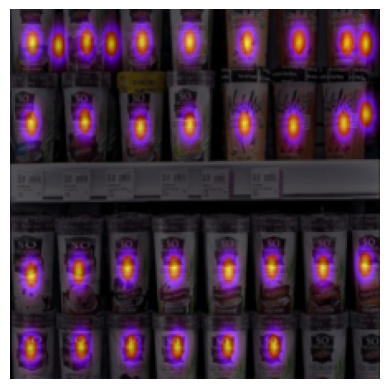
\includegraphics[height=\textwidth,width=\textwidth ]{../files/appendicies/FSC133/images/error_images/too_few/errors_density_maps_3616.png}
 \end{subfigure}
 \begin{subfigure}{0.23\textwidth}
     \centering
    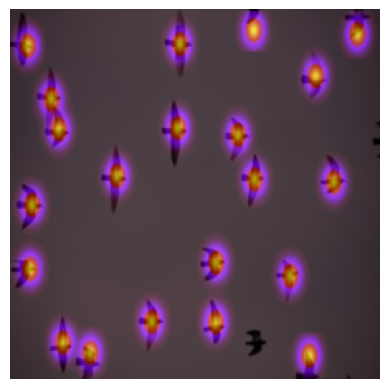
\includegraphics[height=\textwidth,width=\textwidth ]{../files/appendicies/FSC133/images/error_images/too_few/errors_density_maps_394.png}
 \end{subfigure}
 \begin{subfigure}{0.23\textwidth}
     \centering
    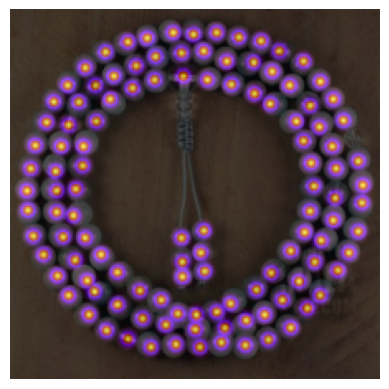
\includegraphics[height=\textwidth,width=\textwidth ]{../files/appendicies/FSC133/images/error_images/too_few/errors_density_maps_4034.png}
 \end{subfigure}\\
  \begin{subfigure}{0.23\textwidth}
     \centering
    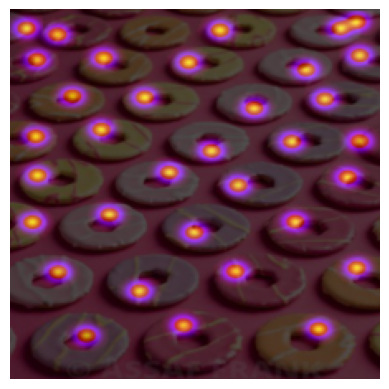
\includegraphics[height=\textwidth,width=\textwidth ]{../files/appendicies/FSC133/images/error_images/too_few/errors_density_maps_4200.png}
 \end{subfigure}
 \begin{subfigure}{0.23\textwidth}
     \centering
    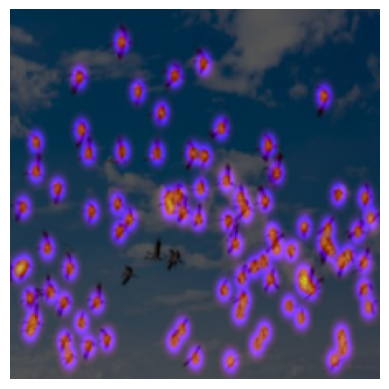
\includegraphics[height=\textwidth,width=\textwidth ]{../files/appendicies/FSC133/images/error_images/too_few/errors_density_maps_4317.png}
 \end{subfigure}
 \begin{subfigure}{0.23\textwidth}
     \centering
    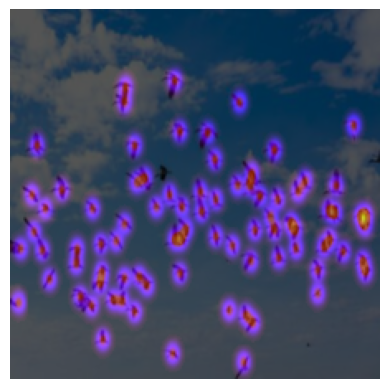
\includegraphics[height=\textwidth,width=\textwidth ]{../files/appendicies/FSC133/images/error_images/too_few/errors_density_maps_4354.png}
 \end{subfigure}\\
 \begin{subfigure}{0.23\textwidth}
     \centering
    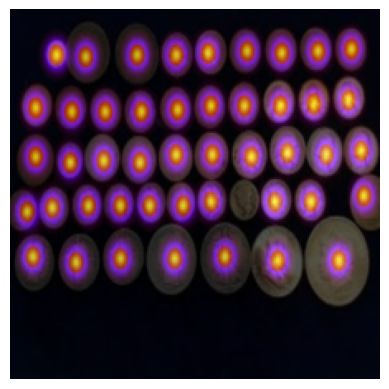
\includegraphics[height=\textwidth,width=\textwidth ]{../files/appendicies/FSC133/images/error_images/too_few/errors_density_maps_7642.png}
 \end{subfigure}
 \begin{subfigure}{0.23\textwidth}
     \centering
    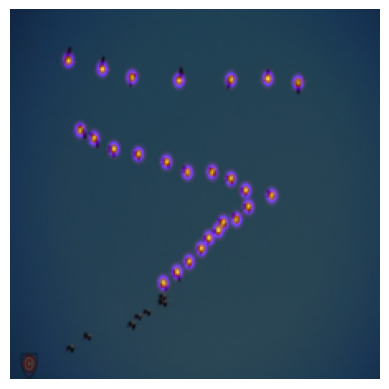
\includegraphics[height=\textwidth,width=\textwidth ]{../files/appendicies/FSC133/images/error_images/too_few/errors_density_maps_4399.png}
 \end{subfigure}
 \begin{subfigure}{0.23\textwidth}
     \centering
    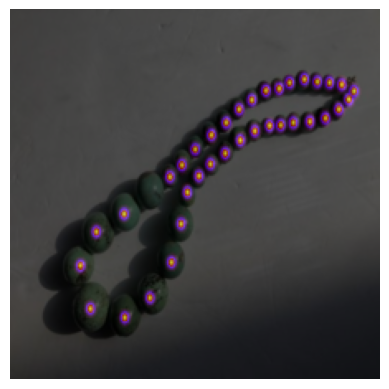
\includegraphics[height=\textwidth,width=\textwidth ]{../files/appendicies/FSC133/images/error_images/too_few/errors_density_maps_5469.png}
 \end{subfigure}\\
  \begin{subfigure}{0.23\textwidth}
     \centering
    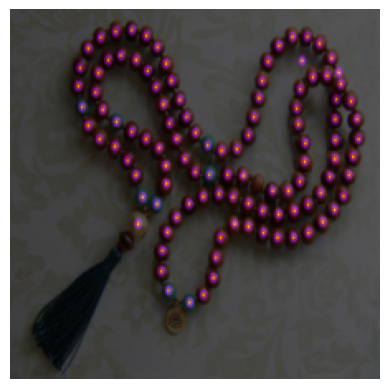
\includegraphics[height=\textwidth,width=\textwidth ]{../files/appendicies/FSC133/images/error_images/too_few/errors_density_maps_5750.png}
 \end{subfigure}
 \begin{subfigure}{0.23\textwidth}
     \centering
    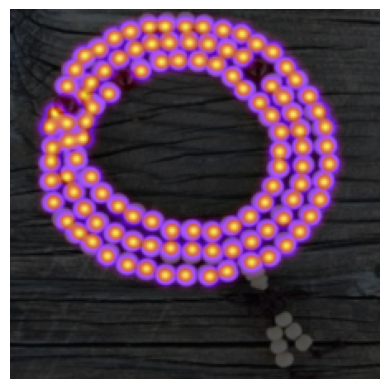
\includegraphics[height=\textwidth,width=\textwidth ]{../files/appendicies/FSC133/images/error_images/too_few/errors_density_maps_5754.png}
 \end{subfigure}
 \begin{subfigure}{0.23\textwidth}
     \centering
    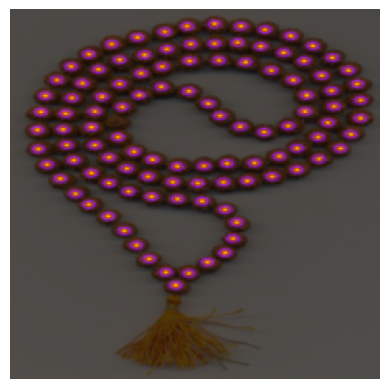
\includegraphics[height=\textwidth,width=\textwidth ]{../files/appendicies/FSC133/images/error_images/too_few/errors_density_maps_6436.png}
 \end{subfigure}\\
 
 \begin{subfigure}{0.23\textwidth}
     \centering
    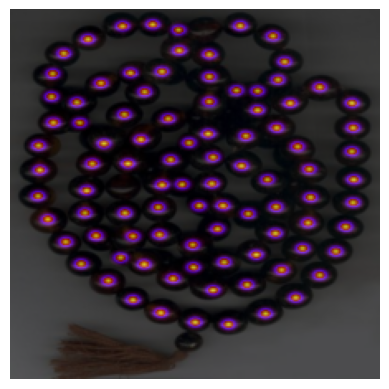
\includegraphics[height=\textwidth,width=\textwidth ]{../files/appendicies/FSC133/images/error_images/too_few/errors_density_maps_6478.png}
 \end{subfigure}
  \begin{subfigure}{0.23\textwidth}
     \centering
    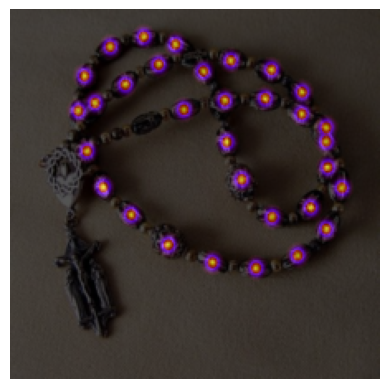
\includegraphics[height=\textwidth,width=\textwidth ]{../files/appendicies/FSC133/images/error_images/too_few/errors_density_maps_6497.png}
 \end{subfigure}
  \begin{subfigure}{0.23\textwidth}
     \centering
    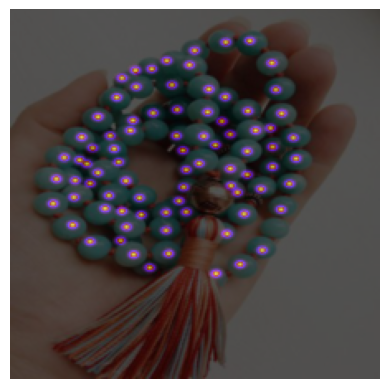
\includegraphics[height=\textwidth,width=\textwidth ]{../files/appendicies/FSC133/images/error_images/too_few/errors_density_maps_6539.png}
 \end{subfigure}\\
 \begin{subfigure}{0.23\textwidth}
     \centering
    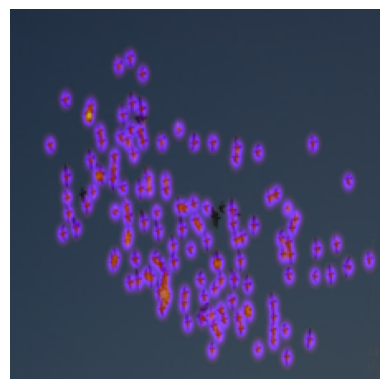
\includegraphics[height=\textwidth,width=\textwidth ]{../files/appendicies/FSC133/images/error_images/too_few/errors_density_maps_6555.png}
 \end{subfigure}
  \begin{subfigure}{0.23\textwidth}
     \centering
    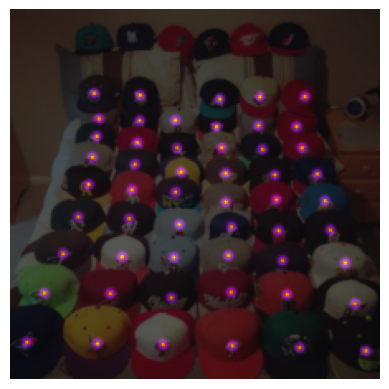
\includegraphics[height=\textwidth,width=\textwidth ]{../files/appendicies/FSC133/images/error_images/too_few/errors_density_maps_6749.png}
 \end{subfigure}
 \begin{subfigure}{0.23\textwidth}
     \centering
    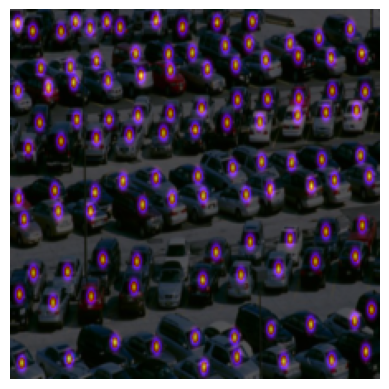
\includegraphics[height=\textwidth,width=\textwidth ]{../files/appendicies/FSC133/images/error_images/too_few/errors_density_maps_6864.png}
 \end{subfigure}\\
 
 
 


 
 
 
    \caption{Examples of cases in the FSC-147  with missing annotations. There are object instances in these images that we believe are semantically similar enough to be included in the count.}
    \label{fig__FSC133__Fig_annotation_errors_missing}
\end{figure}


\begin{figure}     
    \centering
    \fontsize{8}{8}\selectfont
     
 \begin{subfigure}{0.24\textwidth}
     \centering
    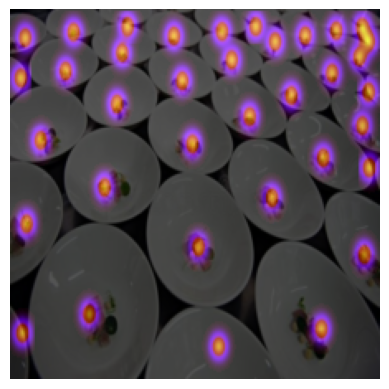
\includegraphics[height=\textwidth,width=\textwidth ]{../files/appendicies/FSC133/images/error_images/too_many/errors_density_maps_900.png}
 \end{subfigure} 
 \begin{subfigure}{0.24\textwidth}
     \centering
    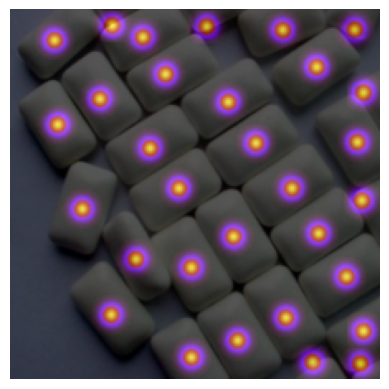
\includegraphics[height=\textwidth,width=\textwidth ]{../files/appendicies/FSC133/images/error_images/too_many/errors_density_maps_3709.png}
 \end{subfigure}
 \begin{subfigure}{0.24\textwidth}
     \centering
    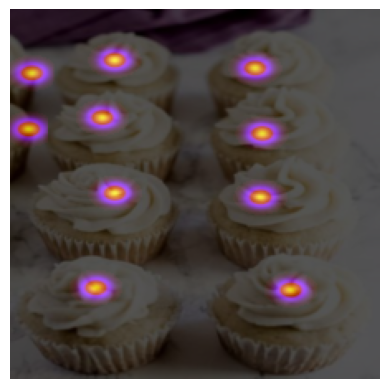
\includegraphics[height=\textwidth,width=\textwidth ]{../files/appendicies/FSC133/images/error_images/too_many/errors_density_maps_3812.png}
 \end{subfigure}\\


  \begin{subfigure}{0.24\textwidth}
     \centering
    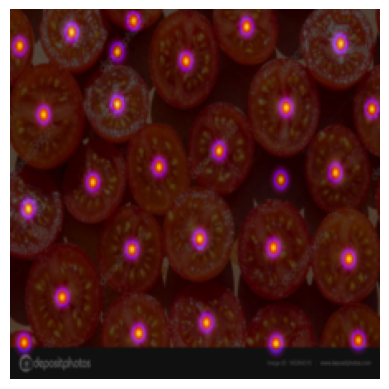
\includegraphics[height=\textwidth,width=\textwidth ]{../files/appendicies/FSC133/images/error_images/too_many/errors_density_maps_4436.png}
 \end{subfigure}
 \begin{subfigure}{0.24\textwidth}
     \centering
    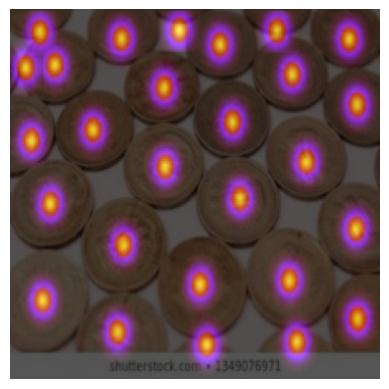
\includegraphics[height=\textwidth,width=\textwidth ]{../files/appendicies/FSC133/images/error_images/too_many/errors_density_maps_6233.png}
 \end{subfigure}
 \begin{subfigure}{0.24\textwidth}
     \centering
    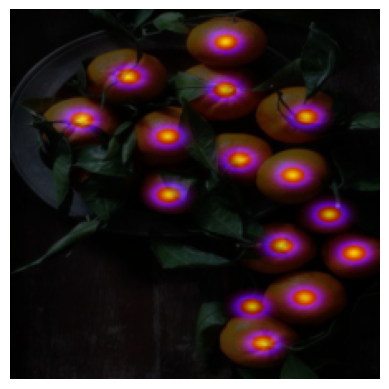
\includegraphics[height=\textwidth,width=\textwidth ]{../files/appendicies/FSC133/images/error_images/too_many/errors_density_maps_6579.png}
 \end{subfigure}\\
 
 \begin{subfigure}{0.24\textwidth}
     \centering
    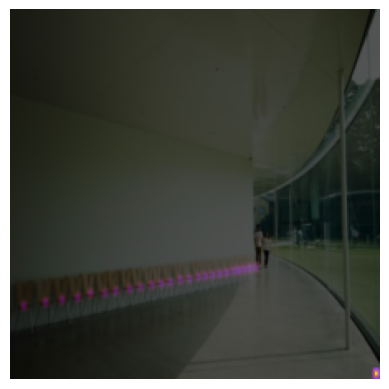
\includegraphics[height=\textwidth,width=\textwidth ]{../files/appendicies/FSC133/images/error_images/too_many/errors_density_maps_2840.png}
 \end{subfigure}
 \begin{subfigure}{0.24\textwidth}
     \centering
    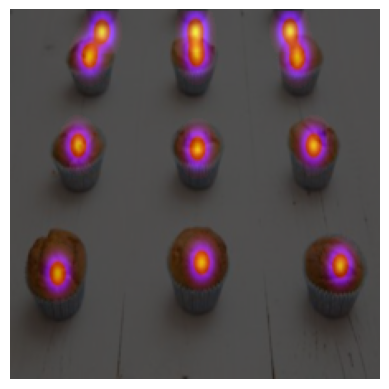
\includegraphics[height=\textwidth,width=\textwidth ]{../files/appendicies/FSC133/images/error_images/too_many/errors_density_maps_3825.png}
 \end{subfigure}
 \begin{subfigure}{0.24\textwidth}
     \centering
    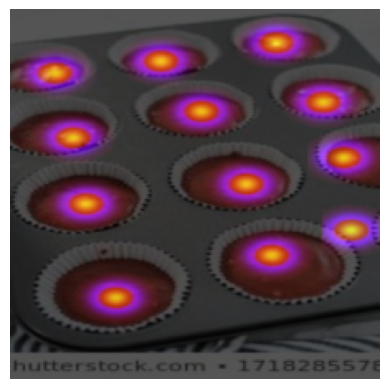
\includegraphics[height=\textwidth,width=\textwidth ]{../files/appendicies/FSC133/images/error_images/too_many/errors_density_maps_5783.png}
 \end{subfigure}\\
  \begin{subfigure}{0.24\textwidth}
     \centering
    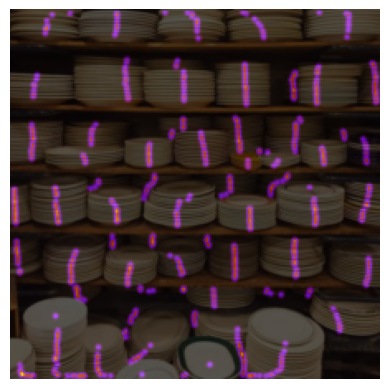
\includegraphics[height=\textwidth,width=\textwidth ]{../files/appendicies/FSC133/images/error_images/too_many/errors_density_maps_880.png}
 \end{subfigure}
  \begin{subfigure}{0.24\textwidth}
     \centering
    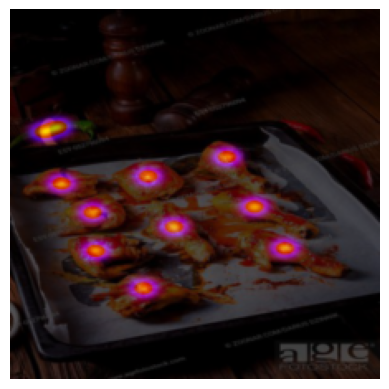
\includegraphics[height=\textwidth,width=\textwidth ]{../files/appendicies/FSC133/images/error_images/too_many/errors_density_maps_3580.png}
 \end{subfigure} 
 \begin{subfigure}{0.24\textwidth}
     \centering
    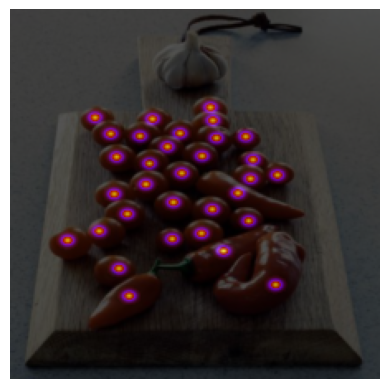
\includegraphics[height=\textwidth,width=\textwidth ]{../files/appendicies/FSC133/images/error_images/too_many/errors_density_maps_70.png}
 \end{subfigure}




    \caption{Examples of cases in FSC-147 with additional instance annotations. These either include highly occluded instances, include annotations for objects of different classes (\eg chilli pepper vs chicken wing), or have erroneous annotations.}
    \label{fig__FSC133__Fig_annotation_errors_additional}
\end{figure}

\begin{figure}     
    \centering
    \fontsize{8}{8}\selectfont
     \begin{subfigure}{0.24\textwidth}
     \centering
    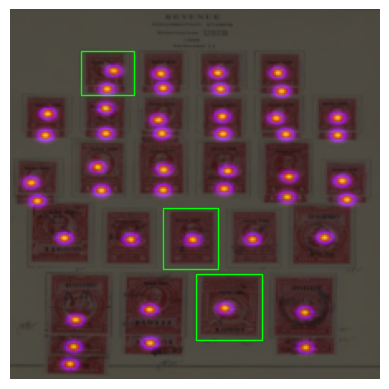
\includegraphics[height=\textwidth,width=\textwidth ]{../files/appendicies/FSC133/images/error_images/ambiguous/3errors_ims_2928.png}
 \end{subfigure}
 \begin{subfigure}{0.24\textwidth}
     \centering
    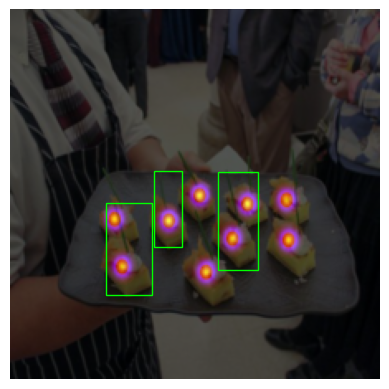
\includegraphics[height=\textwidth,width=\textwidth ]{../files/appendicies/FSC133/images/error_images/ambiguous/3errors_ims_5381.png}
 \end{subfigure}
 \begin{subfigure}{0.24\textwidth}
     \centering
    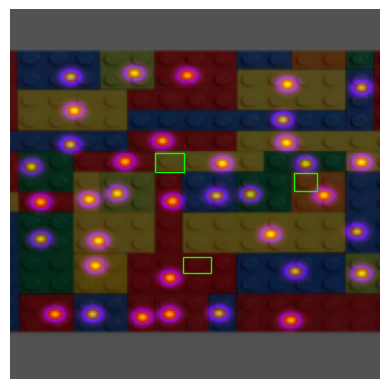
\includegraphics[height=\textwidth,width=\textwidth ]{../files/appendicies/FSC133/images/error_images/ambiguous/3errors_ims_6842.png}
 \end{subfigure}\\
 \begin{subfigure}{0.24\textwidth}
     \centering
    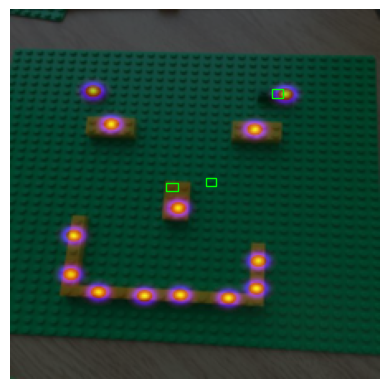
\includegraphics[height=\textwidth,width=\textwidth ]{../files/appendicies/FSC133/images/error_images/ambiguous/3errors_ims_7171.png}
 \end{subfigure}
 \begin{subfigure}{0.24\textwidth}
     \centering
    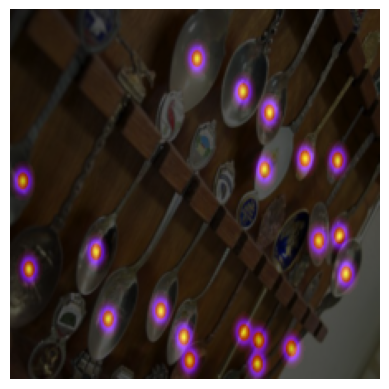
\includegraphics[height=\textwidth,width=\textwidth ]{../files/appendicies/FSC133/images/error_images/ambiguous/errors_density_maps_2522.png}
 \end{subfigure}
 \begin{subfigure}{0.24\textwidth}
     \centering
    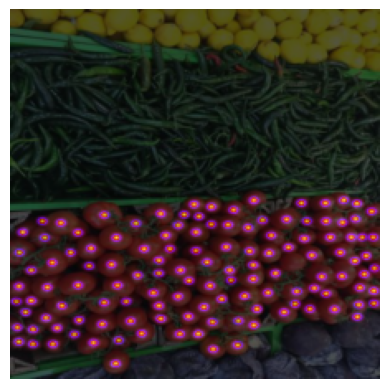
\includegraphics[height=\textwidth,width=\textwidth ]{../files/appendicies/FSC133/images/error_images/ambiguous/errors_density_maps_31.png}
 \end{subfigure}\\
 \begin{subfigure}{0.24\textwidth}
     \centering
    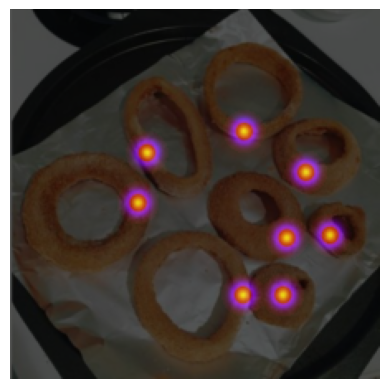
\includegraphics[height=\textwidth,width=\textwidth ]{../files/appendicies/FSC133/images/error_images/ambiguous/errors_density_maps_3346.png}
 \end{subfigure}
 \begin{subfigure}{0.24\textwidth}
     \centering
    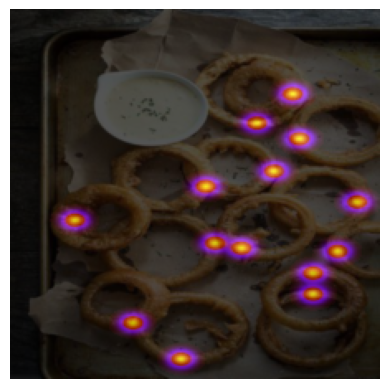
\includegraphics[height=\textwidth,width=\textwidth ]{../files/appendicies/FSC133/images/error_images/ambiguous/errors_density_maps_3347.png}
 \end{subfigure}
 \begin{subfigure}{0.24\textwidth}
     \centering
    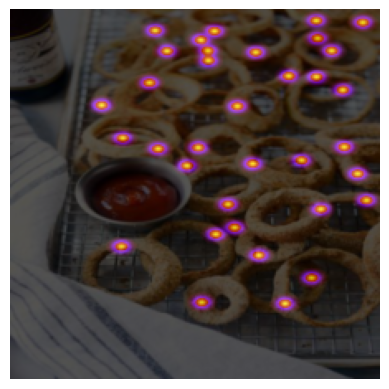
\includegraphics[height=\textwidth,width=\textwidth ]{../files/appendicies/FSC133/images/error_images/ambiguous/errors_density_maps_3348.png}
 \end{subfigure}\\
 

    \caption{Examples of ambiguous annotations  in FSC-147. 
    These include bounding box annotations that include more than one point annotation, point annotations and bounding box annotations defining different classes, arbitrarily selected classes to count, or arbitrarily placed point annotations.
     }
    \label{fig__FSC133__Fig_annotation_errors_ambiguous}
\end{figure}
Annotation errors can be grouped into various categories. We will focus on (i) Missing counts, (ii) Additional counts, and (iii) Ambiguous annotations.
Missing counts are cases where the labels do not include an object that is very similar to those that have been labelled; see 
\Cref{fig__FSC133__Fig_annotation_errors_missing} for examples.
Additional counts are cases where instance annotations are added either to objects that are not semantically similar, to objects that are so occluded as to be not significantly visible in the picture, or to erroneous points; see \Cref{fig__FSC133__Fig_annotation_errors_additional} for examples of each.
There are various cases of ambiguous labels where instance annotations or bounding boxes do not align with each other.
Examples of this include bounding boxes that include more than one instance in situations where this was avoidable, instance annotations associated with highly occluded objects, or bounding box annotations for repeated component parts of objects with instance annotations corresponding to the whole objects; see \Cref{fig__FSC133__Fig_annotation_errors_ambiguous} for examples of each.

Many of the missing or additional annotation cases are due to either a lack of semantic understanding, which causes people to group non-similar objects or ignore similar objects, or difficulties with judging occlusion. 
One of the criteria of the dataset is that images have ``no severe occlusion'' such that it would ``prevent humans from accurately counting the objects'' \cite{ranjan2021Famnet}. 
However, this is subjective, leading to annotation errors. 
The lack of consistency associated with manual counting, especially concerning occluded instances, is especially clear when the same image appears multiple times in the dataset with different associated counts. This phenomenon is further discussed in \Cref{sec__FSC133__errors__countdiscrepancy}.


\subsubsection{Repetition Recognition}
Repeated images in a dataset are problematic for multiple reasons.
The least significant effect is that unbalanced datasets reduce the performance of methods as they are often less generalisable. The most impactful effect occurs when the same image is present during training and evaluation. This undermines the test of a method's generalisability.

We identified repeated images using the L1 pixel-wise difference of the two 8-bit images at a resolution of 224 $\times$ 224 pixels. We manually examined each pairing with a difference of less than 10,000 to assess the similarity. 
This manual stage was needed as many images with low pixel-wise difference were clearly different and many with high difference were clearly the same; see \Cref{fig__FSC133ure__no_similar} and \Cref{fig__FSC133__similar} for examples of each phenomenon. 
The cases where the same image has a high pixel-wise difference generally occurred when the image had been compressed, cropped, translated small amounts, or had a colour filter or watermark added.


\begin{figure}   
    \centering
    
\includegraphics[height=0.19\linewidth,width=0.19\linewidth]{../files/appendicies/FSC133/images/raw_ims/6395.jpg}%

\includegraphics[height=0.19\linewidth,width=0.19\linewidth]{../files/appendicies/FSC133/images/raw_ims/6433.jpg}%

\includegraphics[height=0.19\linewidth,width=0.19\linewidth]{../files/appendicies/FSC133/images/raw_ims/6455.jpg}%

\includegraphics[height=0.19\linewidth,width=0.19\linewidth]{../files/appendicies/FSC133/images/raw_ims/6465.jpg}%

\includegraphics[height=0.19\linewidth,width=0.19\linewidth]{../files/appendicies/FSC133/images/raw_ims/6544.jpg}%
\\
\vspace{-0.15em}
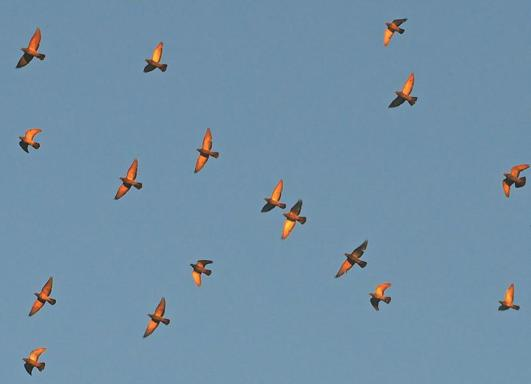
\includegraphics[height=0.19\linewidth,width=0.19\linewidth]{../files/appendicies/FSC133/images/raw_ims/396.jpg}%
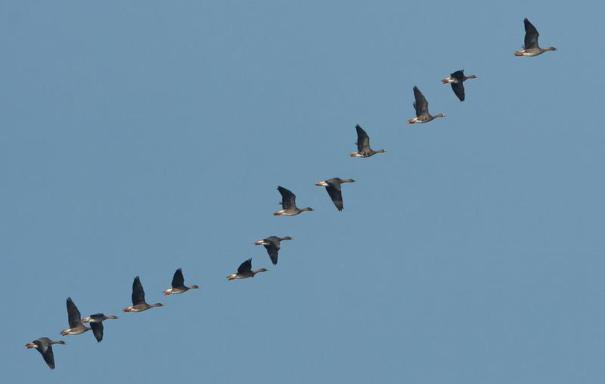
\includegraphics[height=0.19\linewidth,width=0.19\linewidth]{../files/appendicies/FSC133/images/raw_ims/541.jpg}%

\includegraphics[height=0.19\linewidth,width=0.19\linewidth]{../files/appendicies/FSC133/images/white.png}%
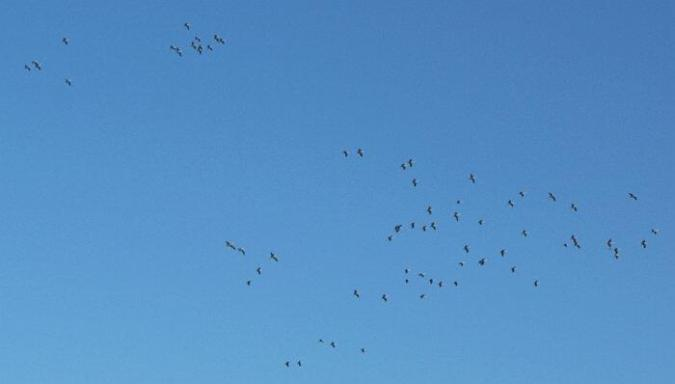
\includegraphics[height=0.19\linewidth,width=0.19\linewidth]{../files/appendicies/FSC133/images/raw_ims/4321.jpg}%
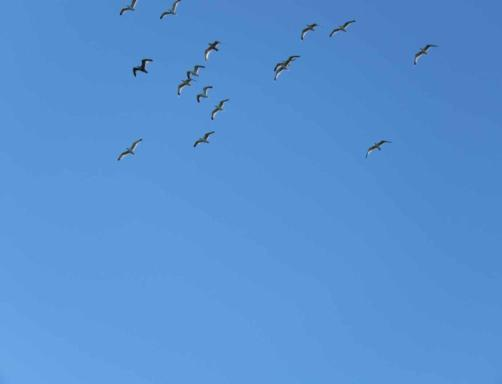
\includegraphics[height=0.19\linewidth,width=0.19\linewidth]{../files/appendicies/FSC133/images/raw_ims/4730.jpg}%
    \caption{Images that have a low pixel-wise difference that we deemed to be different.}
    \label{fig__FSC133ure__no_similar}
\end{figure}

\begin{figure}
    \centering
    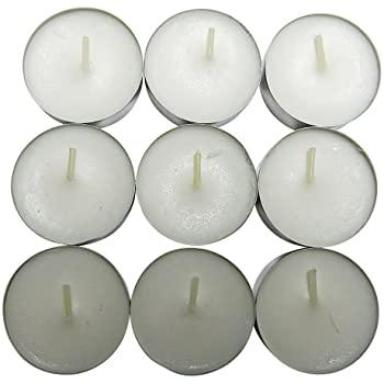
\includegraphics[height=0.19\linewidth, width=0.19\linewidth]{../files/appendicies/FSC133/images/raw_ims/3947.jpg}%
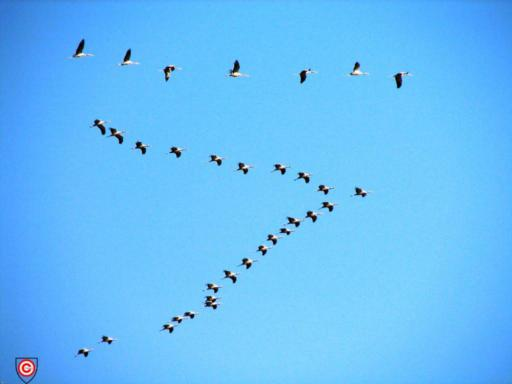
\includegraphics[height=0.19\linewidth, width=0.19\linewidth]{../files/appendicies/FSC133/images/raw_ims/4399.jpg}%

\includegraphics[height=0.19\linewidth, width=0.19\linewidth]{../files/appendicies/FSC133/images/raw_ims/3743.jpg}%

\includegraphics[height=0.19\linewidth, width=0.19\linewidth]{../files/appendicies/FSC133/images/raw_ims/3949.jpg}%

\includegraphics[height=0.19\linewidth, width=0.19\linewidth]{../files/appendicies/FSC133/images/raw_ims/5151.jpg}%
\\
\vspace{-0.0999em}
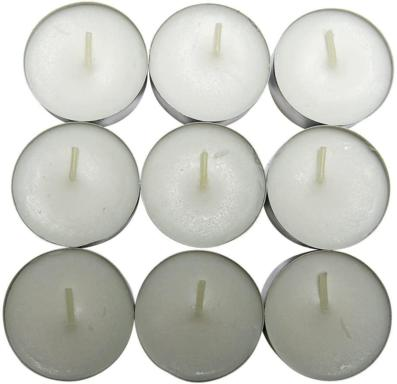
\includegraphics[height=0.19\linewidth, width=0.19\linewidth]{../files/appendicies/FSC133/images/raw_ims/5318.jpg}%
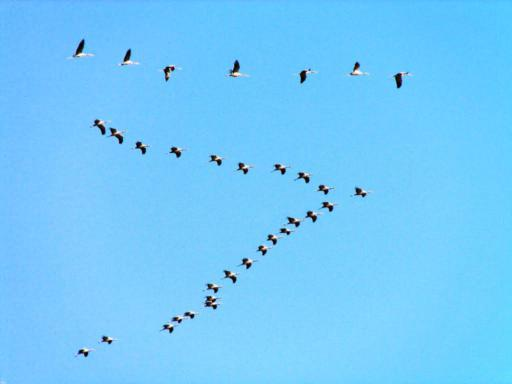
\includegraphics[height=0.19\linewidth, width=0.19\linewidth]{../files/appendicies/FSC133/images/raw_ims/4620.jpg}%
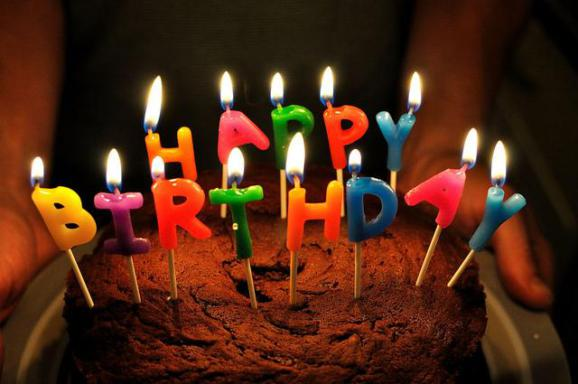
\includegraphics[height=0.19\linewidth, width=0.19\linewidth]{../files/appendicies/FSC133/images/raw_ims/5168.jpg}%
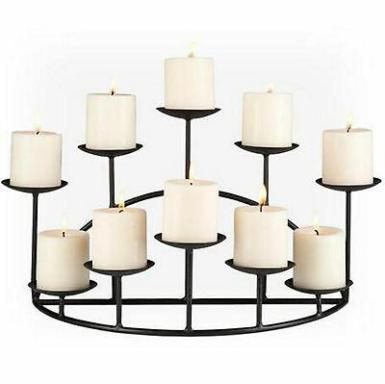
\includegraphics[height=0.19\linewidth, width=0.19\linewidth]{../files/appendicies/FSC133/images/raw_ims/3960.jpg}%

\includegraphics[height=0.19\linewidth, width=0.19\linewidth]{../files/appendicies/FSC133/images/raw_ims/5157.jpg}%
\\

    \caption{Examples of images at the upper bound of pixel-wise difference we considered that we deemed to be the same image. The pixel-wise differences of the images in each column when resized to 224$\times$224 are 5207, 5403, 7551, 8224, and 9396 respectively.}
    \label{fig__FSC133__similar}
\end{figure}


FSC-147 is said to contain 6135 unique images from 147 distinct classes. 
We found that 159 images occur more than once with a pixel-wise difference of 0, for a total of 334 images in the dataset.
If we include images that are close to identical but do not have a zero pixel-wise difference, these numbers increase to 211 images that appear 448 times.
See \Cref{fig__FSC133__subset_dupes} for illustration 
of some of the duplicates.


Not only do some images appear multiple times in the dataset, but 11 images appear in the training set and either the validation set or the testing set; see Table \ref{table__FSC133__FSC_SPLIT_LEAK} for all of the cases. This situation should not be possible as the dataset divisions are made along class boundaries.
Since the purpose of having these splits is to test the ability of a method to generalise to previously unseen classes, this issue is especially significant.

\begin{table}
    \centering
    \resizebox{\textwidth}{!}{%
    \begin{tabular}{clrlclrlrlc}
 \toprule
\multicolumn{4}{c}{Image A} & \multicolumn{4}{c}{Image B} & \multicolumn{2}{c}{Count Diff} \\
ID & Class & Count & Set & Id & Class & Count & Set & Abs & Rel & Kept\\
\cmidrule(r){1-4} \cmidrule(r){5-8} \cmidrule(r){9-10} \cmidrule(r){11-11}

4399 & cranes & 26 & train & 4549 & flamingos & 33 & val & 7 & 0.21 & 4399\\
4399 & cranes & 26 & train & 4719 & seagulls & 33 & val & 7 & 0.21 & 4399 \\
2891 & caps & 144 & train & 1896 & bottle caps & 123 & val & 21 & 0.15 & 1896 \\
4386 & cranes & 20 & train & 7415 & birds & 23 & val & 3 & 0.13 & 4386\\
6567 & pigeons & 21 & train & 929 & birds & 23 & val & 2 & 0.09 & 6567\\
4664 & geese & 11 & train & 6873 & birds & 11 & val & 0 & 0.00 & 4664\\
4613 & geese & 26 & train & 6714 & birds & 26 & val & 0 & 0.00 & 6714\\
4350 & cranes & 8 & train & 4704 & seagulls & 8 & val & 0 & 0.00 & 4683 \\
4350 & cranes & 8 & train & 4707 & seagulls & 8 & val & 0 & 0.00 & 4683\\
3506 & m\&m pieces & 111 & train & 3698 & candy pieces & 111 & test & 0 & 0.00 & 3506\\
3791 & kidney beans & 37 & train & 3494 & red beans & 37 & test & 0 & 0.00 & 3791\\

\bottomrule
\end{tabular}
    }
        \caption{The 17 cases where the same image appears in more than one of the training, validation, or test sets. The right column denotes which of these images (or if a third image) appears in FSC-133.}
    \label{table__FSC133__FSC_SPLIT_LEAK}
\end{table}



Another issue is that there are 71 cases where the same image appears more than once with a different count.
The count discrepancies are up to 25\%, including 5 which appear in both the training set and the validation set with 9\%-21\% discrepancy.
\Cref{fig__FSC133__subset_dupes} presents examples of these errors, and \Cref{table__FSC133__FSC_COUNT_DIFF} contains the complete breakdown of all the cases we found.


\begin{table}
    \centering
    \fontsize{9}{9}\selectfont   
    \resizebox{0.9\textwidth}{!}{%
    \begin{tabular}{rlrlrlrlrrc}
 \toprule
\multicolumn{4}{c}{Image A} & \multicolumn{4}{c}{Image B} & \multicolumn{2}{c}{Count Diff} \\
ID & Class & Count & Set & ID & Class & Count & Set & Abs & Rel & Kept\\
\cmidrule(r){1-4} \cmidrule(r){5-8} \cmidrule(r){9-10} \cmidrule(r){11-11} 
5223 & donuts tray & 9 & val & 5664 & donuts tray & 12 & val & 3 & 25\% & 5223\\
613 & seagulls & 7 & val & 623 & seagulls & 9 & val & 2 & 22\% & 623\\
4399 & cranes & 26 & train & 4549 & flamingos & 33 & val & 7 & 21\% & 4683\\
4399 & cranes & 26 & train & 4620 & geese & 33 & train & 7 & 21\% & 4683\\
4399 & cranes & 26 & train & 4719 & seagulls & 33 & val & 7 & 21\% & 4683\\
3812 & cupcakes & 10 & train & 5238 & cupcakes & 8 & train & 2 & 20\% & 5238 \\
5142 & cashew nuts & 193 & test & 5801 & cashew nuts & 157 & test & 36 & 19\% & 5801\\
4634 & geese & 18 & train & 6143 & geese & 15 & train & 3 & 17\% & 4634\\
4634 & geese & 18 & train & 6669 & geese & 15 & train & 3 & 17\% & 4634 \\
6850 & cereals & 25 & train & 7337 & cereals & 21 & train & 4 & 16\% & 7337\\
6839 & watches & 58 & test & 989 & watches & 69 & test & 11 & 16\% & 6839\\
1896 & bottle caps & 123 & val & 2891 & caps & 144 & train & 21 & 15\% & 1896\\
2717 & oranges & 94 & train & 6573 & oranges & 110 & train & 16 & 15\% & 2717\\
3648 & cashew nuts & 35 & test & 5141 & cashew nuts & 30 & test & 5 & 14\% & 5141\\
3014 & mini blinds & 26 & train & 7307 & mini blinds & 30 & train & 4 & 13\% & 3014 \\
4386 & cranes & 20 & train & 7415 & birds & 23 & val & 3 & 13\% & 4386\\
2970 & fishes & 16 & train & 6953 & fishes & 18 & train & 2 & 11\% & 6953\\
5929 & eggs & 76 & test & 6852 & eggs & 68 & test & 8 & 11\% & 6852\\
4295 & green peas & 110 & test & 5504 & green peas & 122 & test & 12 & 10\% & 4295\\
6567 & pigeons & 21 & train & 929 & birds & 23 & val & 2 &9\% & 6567\\
2743 & oranges & 57 & train & 7363 & oranges & 52 & train & 5 &9\% & 7363\\
6138 & cars & 122 & train & 6864 & cars & 111 & train & 11 &9\% & 6138\\
4220 & biscuits & 11 & train & 5422 & biscuits & 10 & train & 1 &9\% & 5422\\
3282 & finger foods & 31 & test & 3285 & finger foods & 34 & test & 3 &9\% & 3282\\
3462 & beads & 92 & train & 5638 & beads & 85 & train & 7 &8\% & 3462\\
4040 & beads & 117 & train & 5760 & beads & 108 & train & 9 &8\% & 4040\\
3492 & polka dots & 25 & val & 5738 & polka dots & 27 & val & 2 &7\% & 3492\\
3486 & polka dots & 81 & val & 5740 & polka dots & 87 & val & 6 &7\% & 3486\\
6917 & cereals & 29 & train & 7353 & cereals & 27 & train & 2 &7\% & 7353\\
5209 & donuts tray & 17 & val & 5656 & donuts tray & 16 & val & 1 &6\% & 5656\\
4013 & beads & 115 & train & 5754 & beads & 108 & train & 7 &6\% & 5754\\
524 & geese & 30 & train & 635 & cranes & 32 & train & 2 &6\% & 635\\
4300 & green peas & 83 & test & 5506 & green peas & 88 & test & 5 &6\% & 4300\\
3287 & macarons & 16 & train & 428 & macarons & 17 & train & 1 &6\% & 3287\\
4634 & geese & 18 & train & 4675 & geese & 17 & train & 1 &6\% & 4634\\
6602 & pencils & 38 & train & 7400 & pencils & 36 & train & 2 &5\% & 7400\\
3475 & beads & 108 & train & 5637 & beads & 103 & train & 5 &5\% & 3475\\
2357 & bricks & 276 & train & 2401 & bricks & 263 & train & 13 &5\% & 2401\\
4044 & beads & 115 & train & 5335 & beads & 109 & train & 6 &5\% & 4044\\
4019 & beads & 105 & train & 5771 & beads & 109 & train & 4 &4\% & 4019\\
4049 & beads & 26 & train & 5755 & beads & 27 & train & 1 &4\% & 5755\\
3956 & candles & 46 & train & 5309 & candles & 44 & train & 2 &4\% & 5309\\
3969 & candles & 23 & train & 5317 & candles & 24 & train & 1 &4\% & 3969\\
3950 & candles & 24 & train & 5312 & candles & 25 & train & 1 &4\% & 3950\\
3020 & mini blinds & 34 & train & 7630 & mini blinds & 35 & train & 1 &3\% & 3020\\
3668 & toilet paper rolls & 31 & val & 5154 & toilet paper rolls & 32 & val & 1 &3\% & 3668\\
3679 & buns & 35 & train & 5026 & bread rolls & 36 & train & 1 &3\% & 3679\\
4014 & beads & 108 & train & 5749 & beads & 105 & train & 3 &3\% & 4014\\
3645 & cashew nuts & 60 & test & 5797 & cashew nuts & 58 & test & 2 &3\% & 3645\\
5148 & cashew nuts & 36 & test & 5803 & cashew nuts & 35 & test & 1 &3\% & 5148\\
7640 & apples & 32 & test & 7665 & apples & 33 & test & 1 &3\% & 7665\\
3819 & cupcakes & 36 & train & 5241 & cupcakes & 35 & train & 1 &3\% & 5241\\
3754 & pearls & 131 & train & 5185 & pearls & 127 & train & 4 &3\% & 5185\\
3666 & toilet paper rolls & 32 & val & 5157 & toilet paper rolls & 31 & val & 1 &3\% & 5157\\
3639 & jade stones & 31 & train & 5134 & jade stones & 32 & train & 1 &3\% & 3639\\
6200 & coins & 52 & train & 6228 & coins & 53 & train & 1 &2\% & 6200\\
267 & beads & 59 & train & 3242 & beads & 60 & train & 1 &2\% & 267\\
6798 & birds & 87 & val & 976 & birds & 85 & val & 2 &2\% & 976\\
3795 & kidney beans & 53 & train & 5547 & kidney beans & 52 & train & 1 &2\% & 5547\\
3955 & candles & 60 & train & 5306 & candles & 61 & train & 1 &2\% & 3955\\
2671 & bowls & 60 & train & 6724 & bowls & 59 & train & 1 &2\% & 6724\\
6738 & mini blinds & 53 & train & 7130 & mini blinds & 52 & train & 1 &2\% & 7130\\
5053 & beads & 139 & train & 5644 & beads & 136 & train & 3 &2\% & 5644\\
3426 & polka dots & 219 & val & 5046 & polka dots & 215 & val & 4 &2\% & 5046\\
3122 & coffee beans & 90 & train & 3134 & coffee beans & 89 & train & 1 &1\% & 3134\\
6961 & cartridges & 178 & train & 7680 & cartridges & 179 & train & 1 &1\% & 6961\\
4016 & beads & 109 & train & 5333 & beads & 108 & train & 1 &1\% & 5333\\
3469 & beads & 74 & train & 5050 & beads & 75 & train & 1 &1\% & 3469\\
4021 & beads & 106 & train & 5759 & beads & 107 & train & 1 &1\% & 5759\\
5149 & cashew nuts & 111 & test & 5807 & cashew nuts & 110 & test & 1 &1\% & 5807\\
4044 & beads & 115 & train & 5767 & beads & 116 & train & 1 &1\% & 4044\\
\bottomrule
\end{tabular}

    }
     \caption{The 71 cases where the same image appears more than once in FSC-147 with different associated counts. The right column denotes which of these images (or, in some cases a third image) appears in FSC-133.}
    \label{table__FSC133__FSC_COUNT_DIFF}
\end{table}


We believe these errors stem from the fact the images in FSC-147 were scraped from Flickr, Google, and Bing search engines and then manually annotated \cite{ranjan2021Famnet}. 
We assume the images appeared on either multiple sources or were duplicated from the same source. 


\subsubsection{Split overlap}
While images appearing in both the training and evaluation sets would be a problem for any machine learning application, it is especially impactful to the evaluation of class-agnostic counting methods.
To facilitate testing a method's generalisability, the data splits are along class boundaries.
Images that are incorrectly classified can end up in the wrong data split and harm the reliability of this evaluation. 


\begin{figure}    
    \centering
    \fontsize{8}{8}\selectfont
    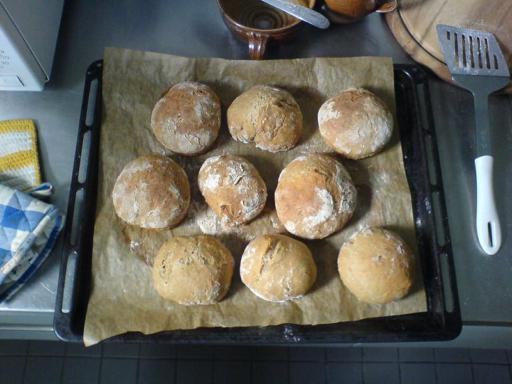
\includegraphics[height=0.1\textwidth,width=0.1\textwidth ]{../files/appendicies/FSC133/images/raw_ims/19.jpg}%
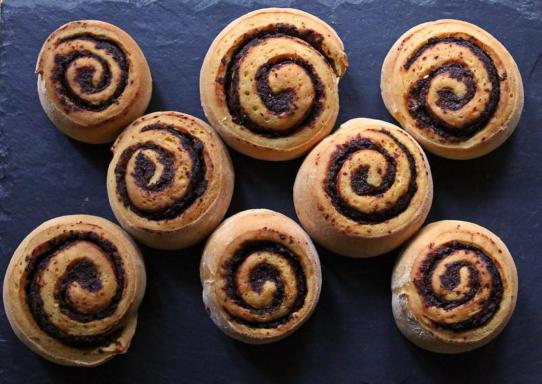
\includegraphics[height=0.1\textwidth,width=0.1\textwidth ]{../files/appendicies/FSC133/images/raw_ims/28.jpg}%
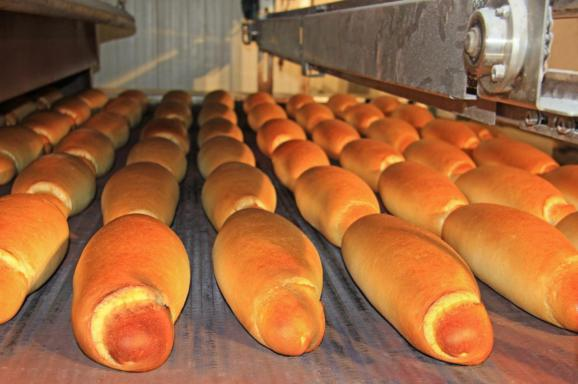
\includegraphics[height=0.1\textwidth,width=0.1\textwidth ]{../files/appendicies/FSC133/images/raw_ims/3381.jpg}%
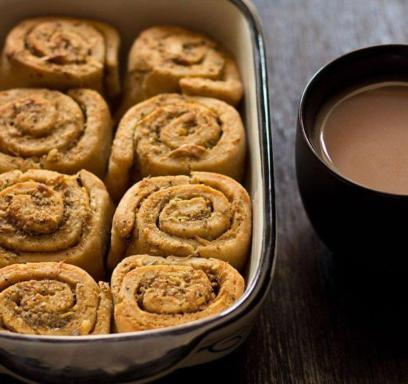
\includegraphics[height=0.1\textwidth,width=0.1\textwidth ]{../files/appendicies/FSC133/images/raw_ims/3394.jpg}%
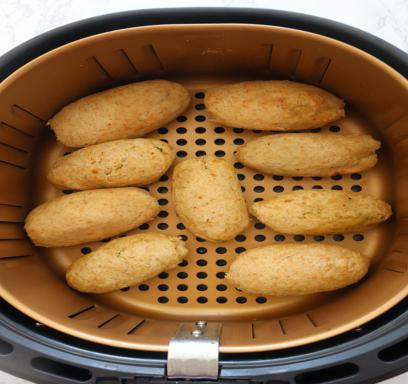
\includegraphics[height=0.1\textwidth,width=0.1\textwidth ]{../files/appendicies/FSC133/images/raw_ims/5966.jpg}%

\includegraphics[height=0.1\textwidth,width=0.1\textwidth ]{../files/appendicies/FSC133/images/raw_ims/5974.jpg}%
\\ \vspace{0.2em}
 Bread Rolls (Train)\\ \vspace{0.2em}
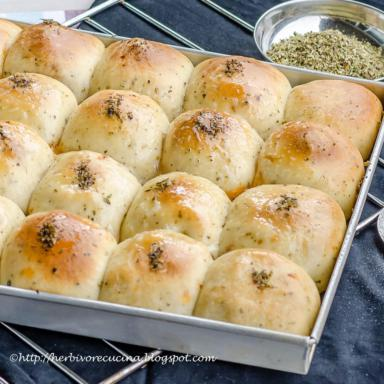
\includegraphics[height=0.1\textwidth,width=0.1\textwidth ]{../files/appendicies/FSC133/images/raw_ims/3676.jpg}%
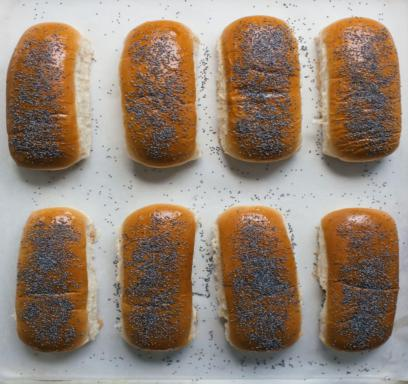
\includegraphics[height=0.1\textwidth,width=0.1\textwidth ]{../files/appendicies/FSC133/images/raw_ims/3681.jpg}%
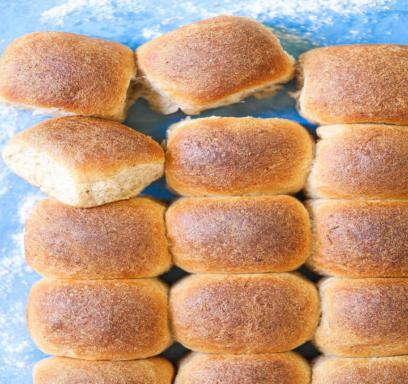
\includegraphics[height=0.1\textwidth,width=0.1\textwidth ]{../files/appendicies/FSC133/images/raw_ims/3684.jpg}%
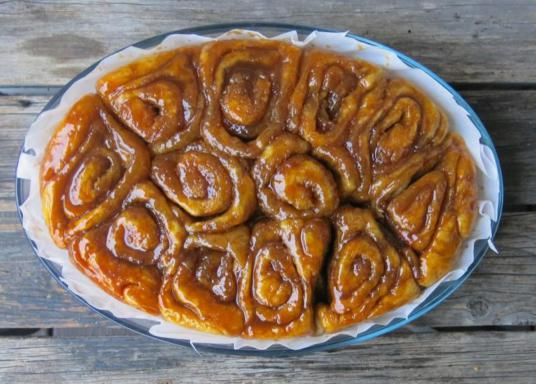
\includegraphics[height=0.1\textwidth,width=0.1\textwidth ]{../files/appendicies/FSC133/images/raw_ims/3685.jpg}%
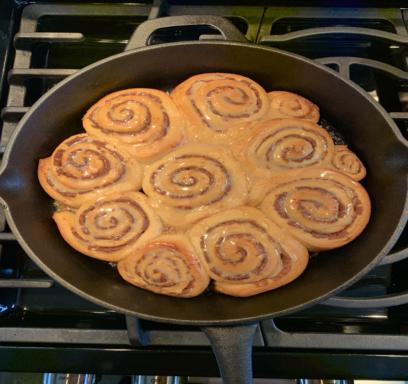
\includegraphics[height=0.1\textwidth,width=0.1\textwidth ]{../files/appendicies/FSC133/images/raw_ims/3691.jpg}%
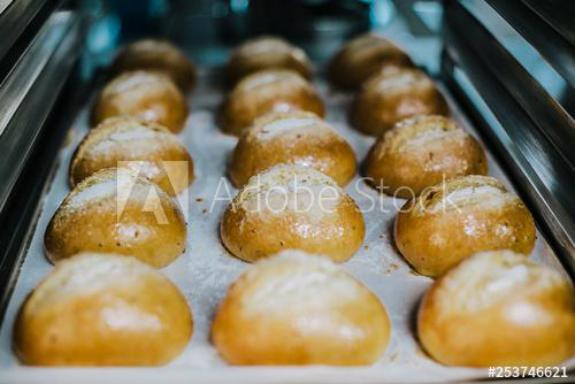
\includegraphics[height=0.1\textwidth,width=0.1\textwidth ]{../files/appendicies/FSC133/images/raw_ims/3680.jpg}%
\\ \vspace{0.2em}
 Buns (Train)\\
 \vspace{0.2em}
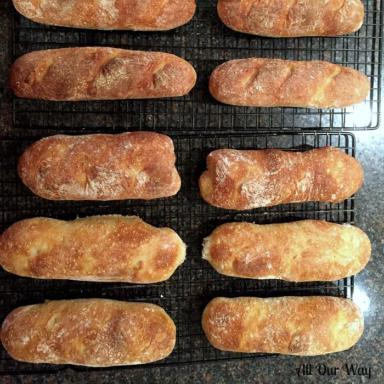
\includegraphics[height=0.1\textwidth,width=0.1\textwidth ]{../files/appendicies/FSC133/images/raw_ims/3511.jpg}%
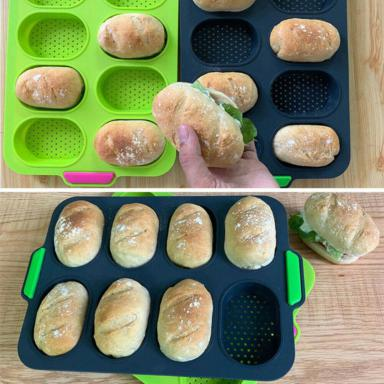
\includegraphics[height=0.1\textwidth,width=0.1\textwidth ]{../files/appendicies/FSC133/images/raw_ims/3512.jpg}%
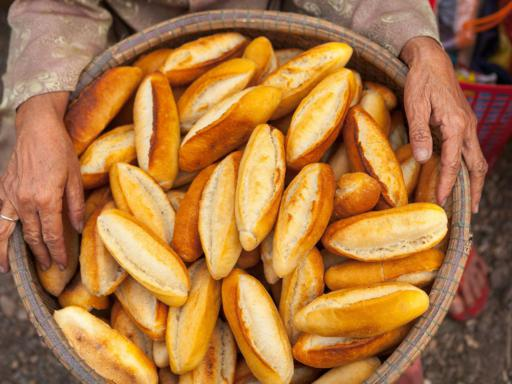
\includegraphics[height=0.1\textwidth,width=0.1\textwidth ]{../files/appendicies/FSC133/images/raw_ims/3514.jpg}%
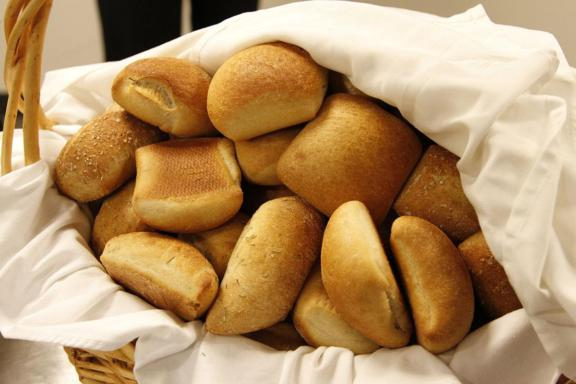
\includegraphics[height=0.1\textwidth,width=0.1\textwidth ]{../files/appendicies/FSC133/images/raw_ims/3515.jpg}%
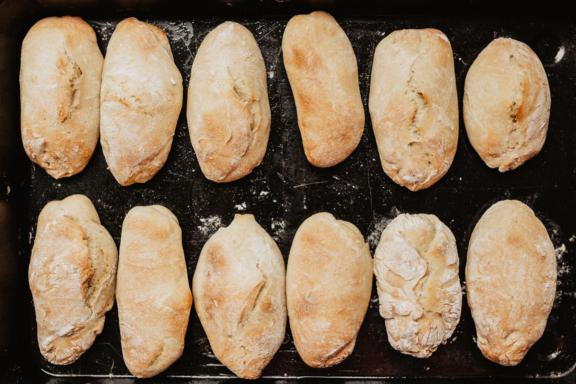
\includegraphics[height=0.1\textwidth,width=0.1\textwidth ]{../files/appendicies/FSC133/images/raw_ims/3516.jpg}%

\includegraphics[height=0.1\textwidth,width=0.1\textwidth ]{../files/appendicies/FSC133/images/white.png}%
\\  \vspace{0.2em}

 Baguette Rolls (Train)\\ \vspace{0.2em}
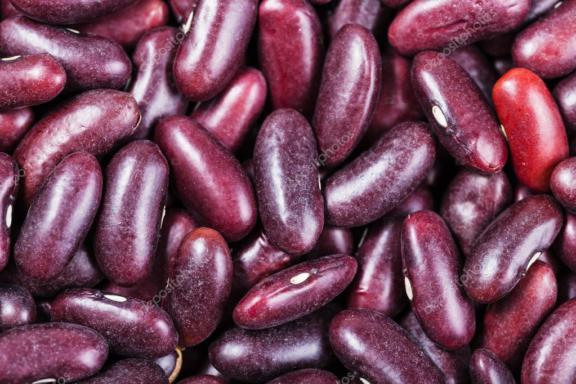
\includegraphics[height=0.1\textwidth,width=0.1\textwidth ]{../files/appendicies/FSC133/images/raw_ims/3493.jpg}%
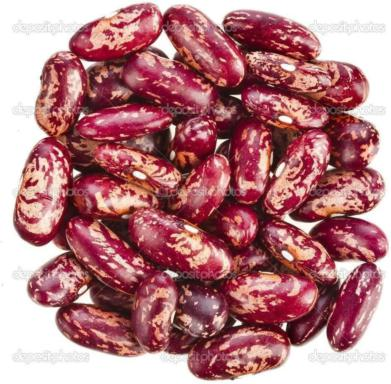
\includegraphics[height=0.1\textwidth,width=0.1\textwidth ]{../files/appendicies/FSC133/images/raw_ims/3494.jpg}%
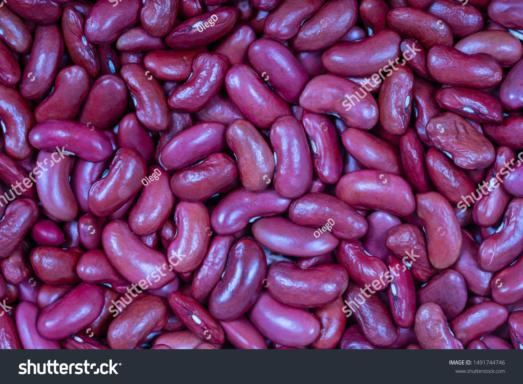
\includegraphics[height=0.1\textwidth,width=0.1\textwidth ]{../files/appendicies/FSC133/images/raw_ims/3495.jpg}%
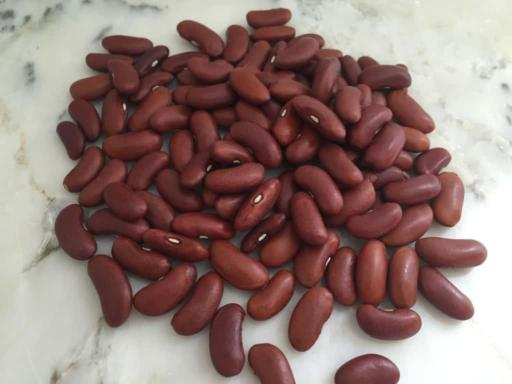
\includegraphics[height=0.1\textwidth,width=0.1\textwidth ]{../files/appendicies/FSC133/images/raw_ims/3498.jpg}%
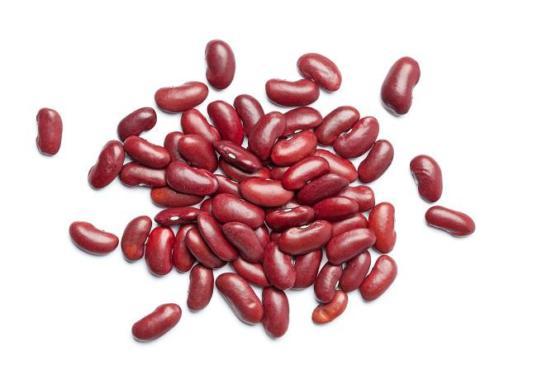
\includegraphics[height=0.1\textwidth,width=0.1\textwidth ]{../files/appendicies/FSC133/images/raw_ims/3501.jpg}%

\includegraphics[height=0.1\textwidth,width=0.1\textwidth ]{../files/appendicies/FSC133/images/raw_ims/3502.jpg}%
\\  \vspace{0.2em}
 Red Beans (Test)\\  \vspace{0.2em}
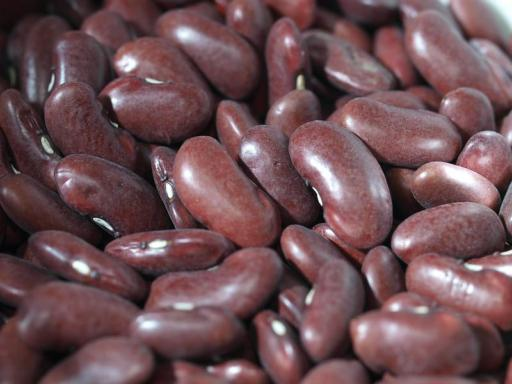
\includegraphics[height=0.1\textwidth,width=0.1\textwidth ]{../files/appendicies/FSC133/images/raw_ims/3224.jpg}%
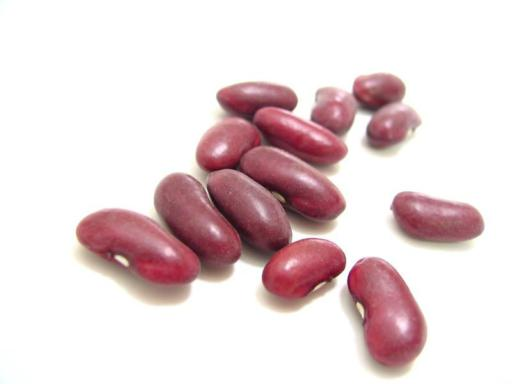
\includegraphics[height=0.1\textwidth,width=0.1\textwidth ]{../files/appendicies/FSC133/images/raw_ims/3227.jpg}%
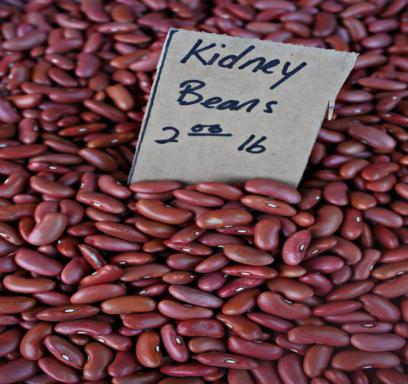
\includegraphics[height=0.1\textwidth,width=0.1\textwidth ]{../files/appendicies/FSC133/images/raw_ims/3231.jpg}%
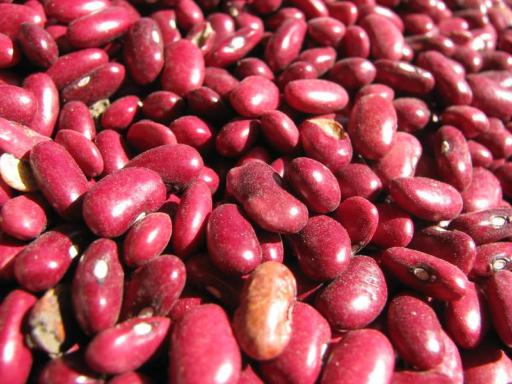
\includegraphics[height=0.1\textwidth,width=0.1\textwidth ]{../files/appendicies/FSC133/images/raw_ims/3233.jpg}%
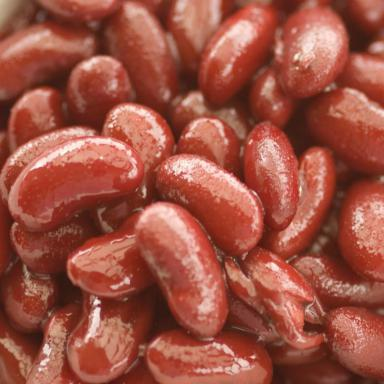
\includegraphics[height=0.1\textwidth,width=0.1\textwidth ]{../files/appendicies/FSC133/images/raw_ims/3234.jpg}%
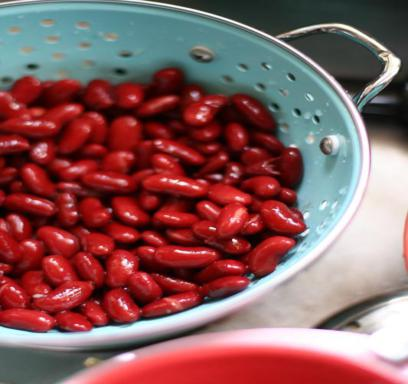
\includegraphics[height=0.1\textwidth,width=0.1\textwidth ]{../files/appendicies/FSC133/images/raw_ims/3235.jpg}%
\\  \vspace{0.2em}
 Kidney Beans (Train)\\  \vspace{0.2em}
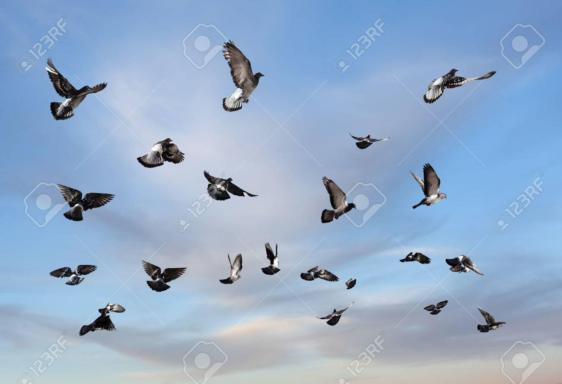
\includegraphics[height=0.1\textwidth,width=0.1\textwidth ]{../files/appendicies/FSC133/images/raw_ims/929.jpg}%
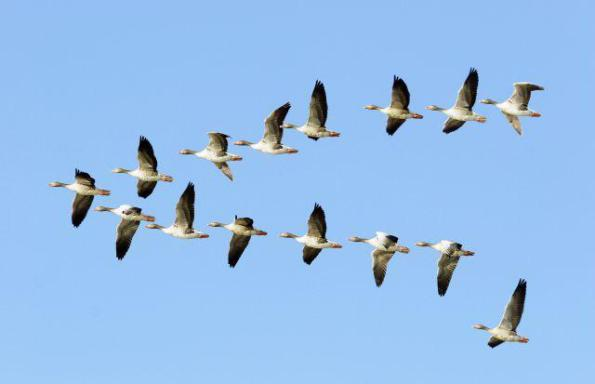
\includegraphics[height=0.1\textwidth,width=0.1\textwidth ]{../files/appendicies/FSC133/images/raw_ims/930.jpg}%
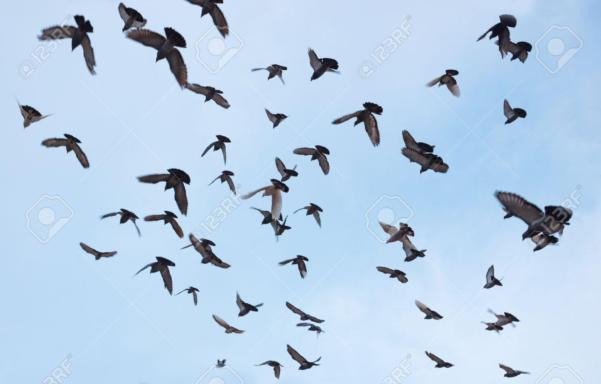
\includegraphics[height=0.1\textwidth,width=0.1\textwidth ]{../files/appendicies/FSC133/images/raw_ims/932.jpg}%
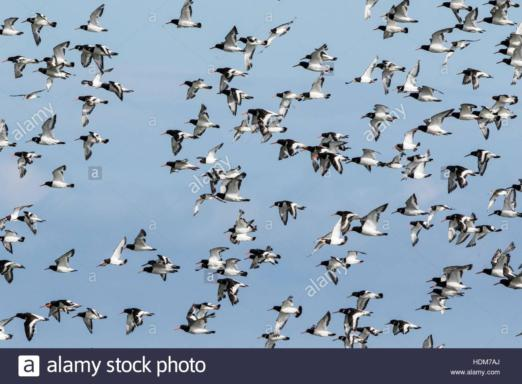
\includegraphics[height=0.1\textwidth,width=0.1\textwidth ]{../files/appendicies/FSC133/images/raw_ims/945.jpg}%
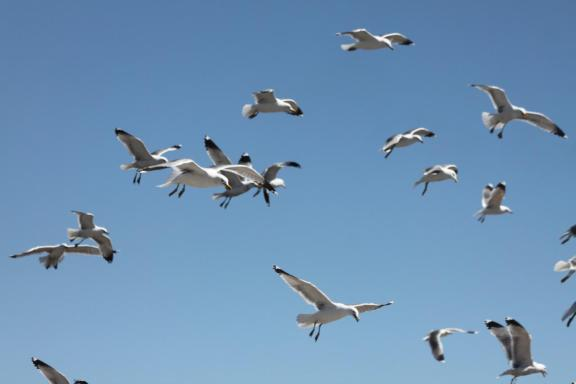
\includegraphics[height=0.1\textwidth,width=0.1\textwidth ]{../files/appendicies/FSC133/images/raw_ims/959.jpg}%
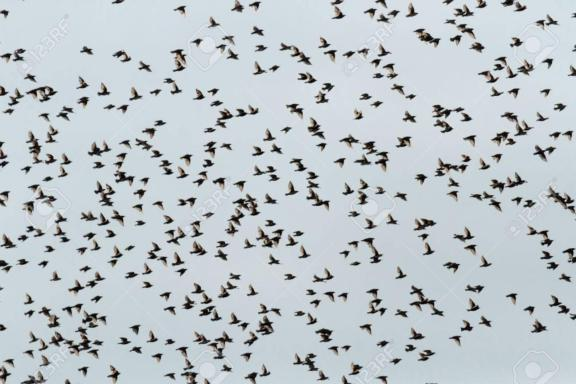
\includegraphics[height=0.1\textwidth,width=0.1\textwidth ]{../files/appendicies/FSC133/images/raw_ims/972.jpg}%
\\  \vspace{0.2em}
 Birds (Val)\\  \vspace{0.2em}
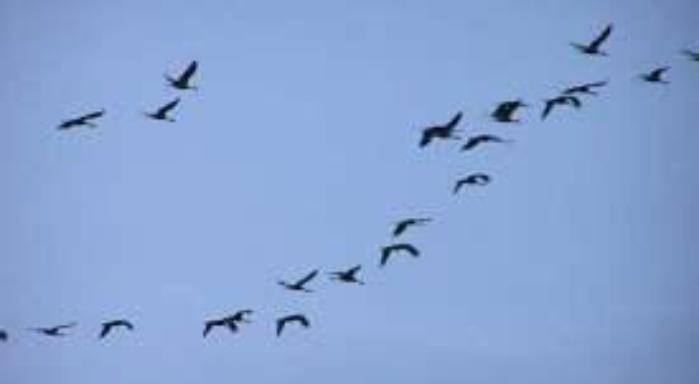
\includegraphics[height=0.1\textwidth,width=0.1\textwidth ]{../files/appendicies/FSC133/images/raw_ims/5953.jpg}%
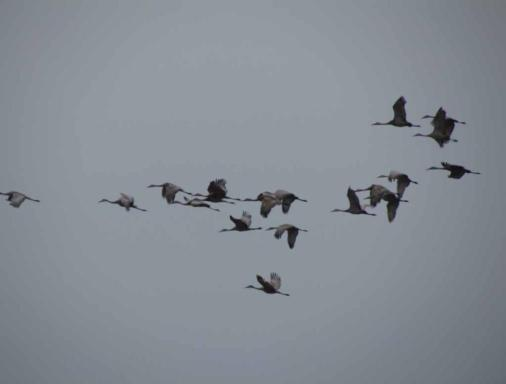
\includegraphics[height=0.1\textwidth,width=0.1\textwidth ]{../files/appendicies/FSC133/images/raw_ims/5954.jpg}%
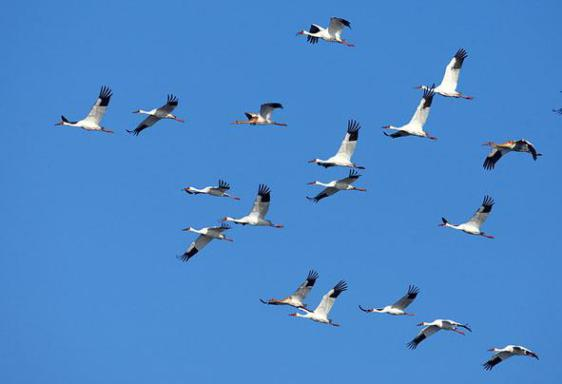
\includegraphics[height=0.1\textwidth,width=0.1\textwidth ]{../files/appendicies/FSC133/images/raw_ims/5956.jpg}%
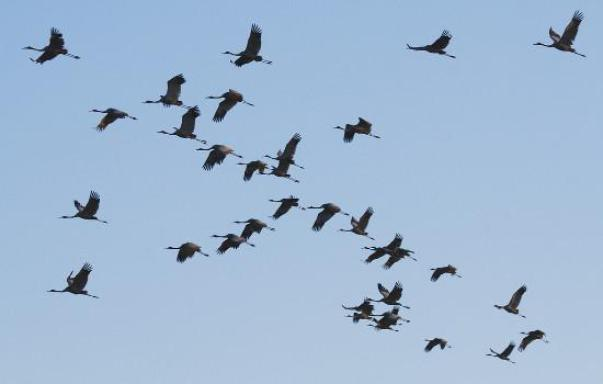
\includegraphics[height=0.1\textwidth,width=0.1\textwidth ]{../files/appendicies/FSC133/images/raw_ims/5957.jpg}%
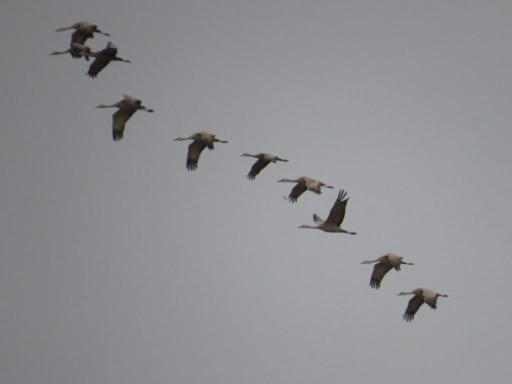
\includegraphics[height=0.1\textwidth,width=0.1\textwidth ]{../files/appendicies/FSC133/images/raw_ims/5959.jpg}%
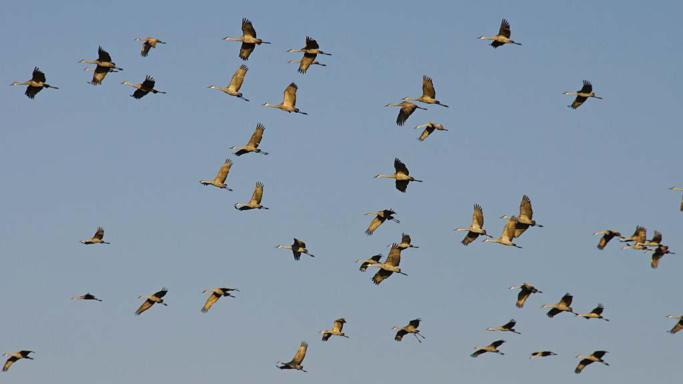
\includegraphics[height=0.1\textwidth,width=0.1\textwidth ]{../files/appendicies/FSC133/images/raw_ims/5960.jpg}%
\\  \vspace{0.2em}
 Cranes (Train)\\  \vspace{0.2em}
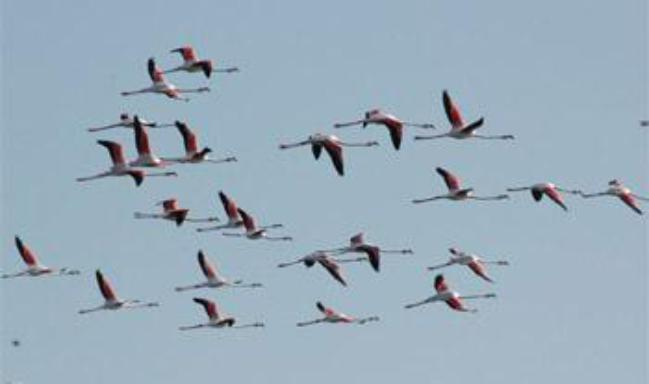
\includegraphics[height=0.1\textwidth,width=0.1\textwidth ]{../files/appendicies/FSC133/images/raw_ims/6070.jpg}%
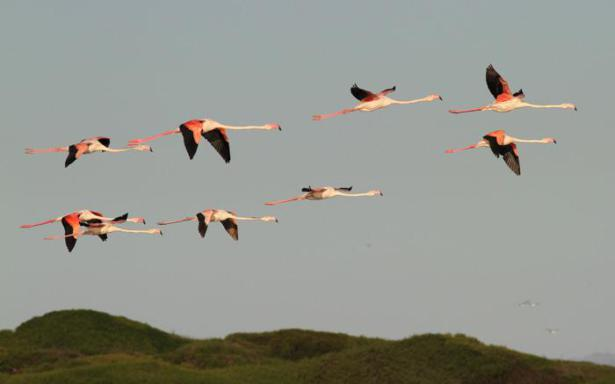
\includegraphics[height=0.1\textwidth,width=0.1\textwidth ]{../files/appendicies/FSC133/images/raw_ims/6071.jpg}%
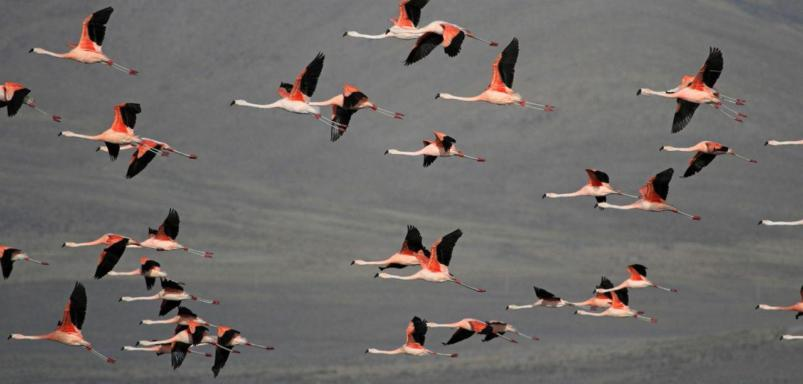
\includegraphics[height=0.1\textwidth,width=0.1\textwidth ]{../files/appendicies/FSC133/images/raw_ims/6072.jpg}%
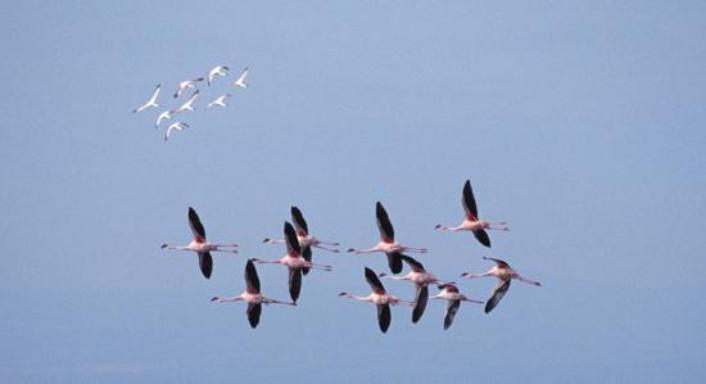
\includegraphics[height=0.1\textwidth,width=0.1\textwidth ]{../files/appendicies/FSC133/images/raw_ims/6073.jpg}%
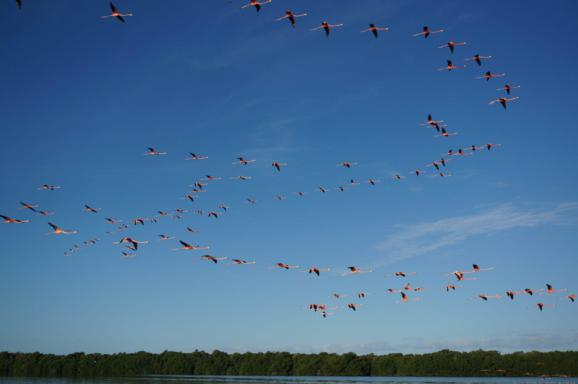
\includegraphics[height=0.1\textwidth,width=0.1\textwidth ]{../files/appendicies/FSC133/images/raw_ims/6075.jpg}%
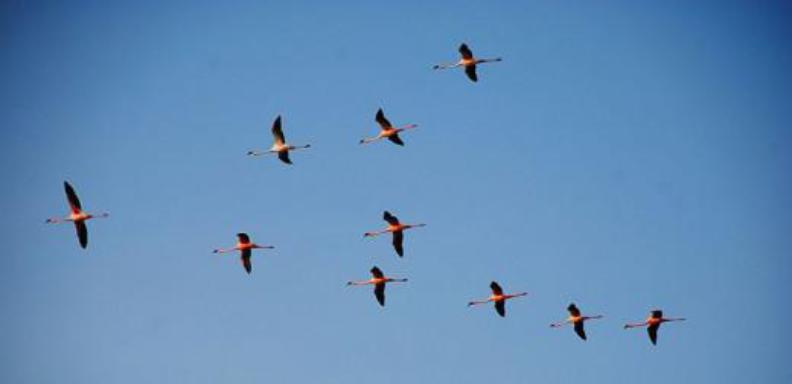
\includegraphics[height=0.1\textwidth,width=0.1\textwidth ]{../files/appendicies/FSC133/images/raw_ims/6079.jpg}%
\\  \vspace{0.2em}
 Flamingos (Val)\\  \vspace{0.2em}
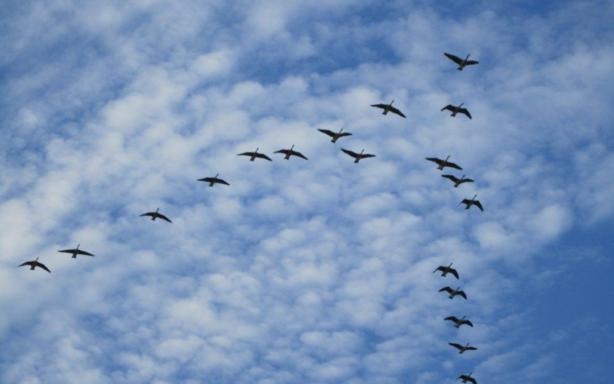
\includegraphics[height=0.1\textwidth,width=0.1\textwidth ]{../files/appendicies/FSC133/images/raw_ims/4612.jpg}%
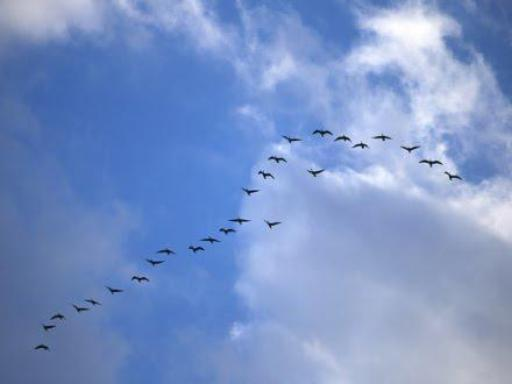
\includegraphics[height=0.1\textwidth,width=0.1\textwidth ]{../files/appendicies/FSC133/images/raw_ims/4613.jpg}%
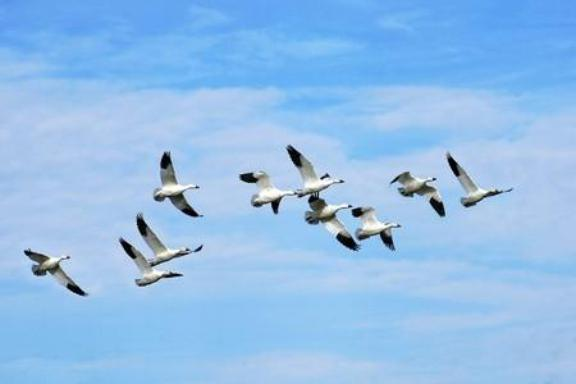
\includegraphics[height=0.1\textwidth,width=0.1\textwidth ]{../files/appendicies/FSC133/images/raw_ims/4615.jpg}%
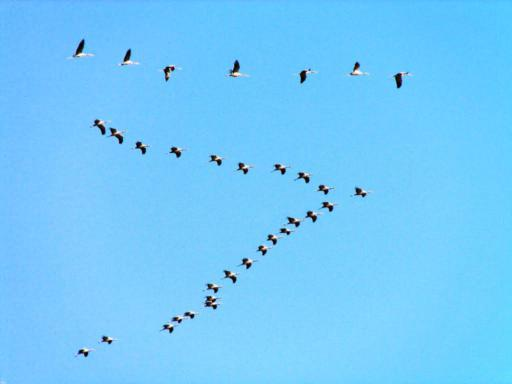
\includegraphics[height=0.1\textwidth,width=0.1\textwidth ]{../files/appendicies/FSC133/images/raw_ims/4620.jpg}%
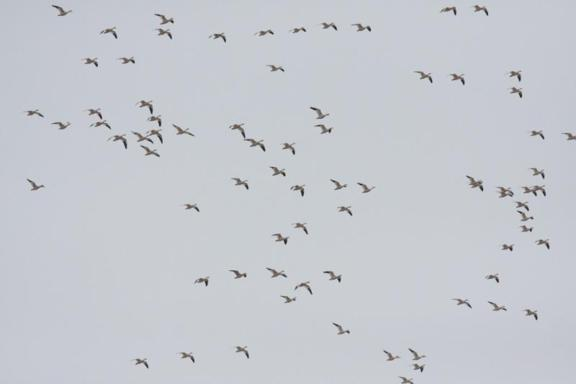
\includegraphics[height=0.1\textwidth,width=0.1\textwidth ]{../files/appendicies/FSC133/images/raw_ims/4627.jpg}%
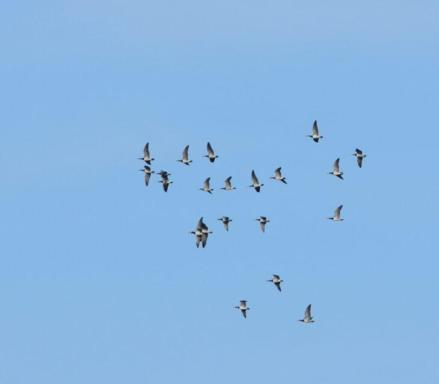
\includegraphics[height=0.1\textwidth,width=0.1\textwidth ]{../files/appendicies/FSC133/images/raw_ims/4628.jpg}%
\\  \vspace{0.2em}
 Geese (Train)\\  \vspace{0.2em}
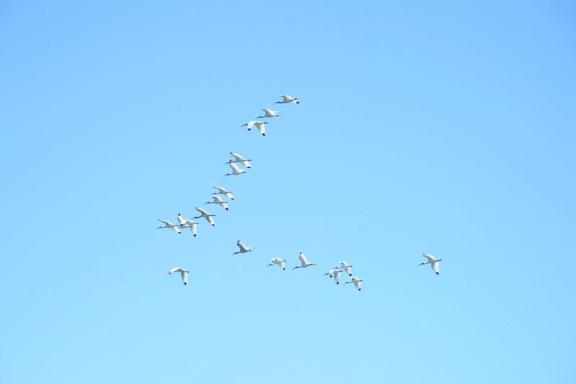
\includegraphics[height=0.1\textwidth,width=0.1\textwidth ]{../files/appendicies/FSC133/images/raw_ims/192.jpg}%
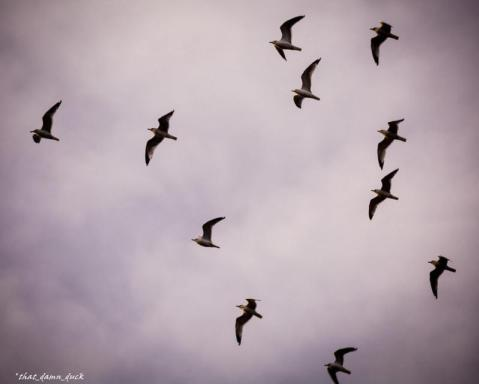
\includegraphics[height=0.1\textwidth,width=0.1\textwidth ]{../files/appendicies/FSC133/images/raw_ims/591.jpg}%
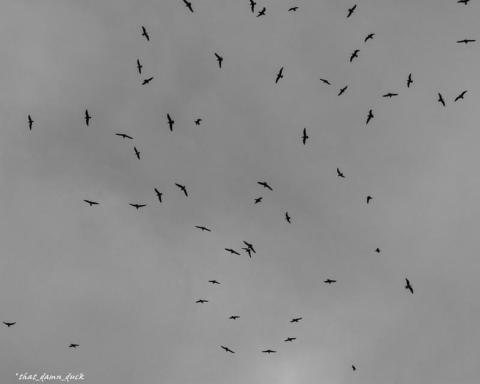
\includegraphics[height=0.1\textwidth,width=0.1\textwidth ]{../files/appendicies/FSC133/images/raw_ims/597.jpg}%
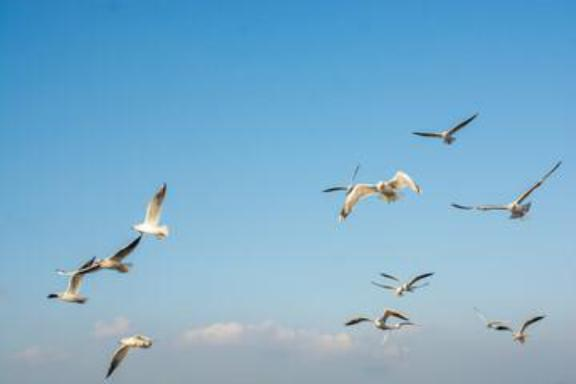
\includegraphics[height=0.1\textwidth,width=0.1\textwidth ]{../files/appendicies/FSC133/images/raw_ims/4703.jpg}%
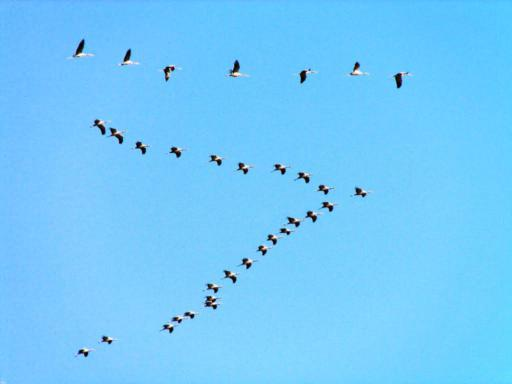
\includegraphics[height=0.1\textwidth,width=0.1\textwidth ]{../files/appendicies/FSC133/images/raw_ims/4719.jpg}%
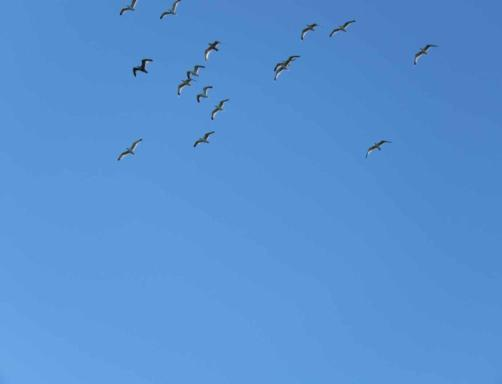
\includegraphics[height=0.1\textwidth,width=0.1\textwidth ]{../files/appendicies/FSC133/images/raw_ims/4730.jpg}%
\\
Seagulls (Val)\\  \vspace{0.2em}
    \caption{Examples of clear overlap or similarity between classes. Each row has a different class label in FSC-147. In FSC-133, these are simplified to Bread Rolls (Train), Kidney Beans (Train), and Birds (Train).}
    \label{fig__FSC133__arethesame}
\end{figure}

There are a few instances in FSC-147  where images are clearly incorrectly classified. 
Some of these errors are obvious and stem from a misapplication of the class labels.
For example, `bottle caps' being classified as `caps', a category designed for baseball caps. 
However, the majority of incorrect classifications stem from ambiguities in the class labels.
FSC-147 has sets of classes which are visually very similar such as `red beans (test)' and `kidney beans (train)' or many of the bird classes.
Identifying the bird classes is particularly challenging as it is difficult to recognise which of the categories is present when the instances are small or in silhouette.
There are also hierarchical arrangements of classes. 
For example, `cranes (train)', `seagulls (val)', and `geese (train)' could all also be classified as `birds (val)', and `buns (train)' and `baguette rolls (train)' could also be classified as `bread rolls (train)'. 
See \Cref{fig__FSC133__arethesame} for visual examples of these similarities.

These errors could occur when there is a language, expertise, or cultural difference in the labelling population. For example, `Cranes' and `geese' look very similar. Presented with an image and a set of ambiguous class labels, a human annotator may well assume the image is of the type with which they are more familiar. 
Similarly, the `bread rolls', `buns', and `baguette rolls' categories depend on a linguistic and cultural understanding of the difference between these categories. 
We suggest combining categories that are similar enough that they could be easily mistaken for each other. This is both to disambiguate the dataset but also because we believe they do not fit the `few-shot counting' description, \eg training on images of geese in silhouette against a blue sky and then evaluating on cranes in silhouette against a blue sky is not a good test of the generalisability of a method.

\subsubsection{Count discrepancy}\label{sec__FSC133__errors__countdiscrepancy}
As there is no rigorous way to determine the occlusion of objects from scraped images,  there is no rigorous way of deciding if an instance should be included in the count or not.
When an object is occluded by either another object or the boundary of the image, it is subjective whether that object is `worth counting', which can lead to inconsistent labelling.
This subjectivity is particularly highlighted when the same image appears more than once with a difference in the associated count value.
Figure \ref{fig__FSC133__subset_dupes} shows examples of some of the cases where the same image appears with a discrepancy in the count and \Cref{table__FSC133__FSC_COUNT_DIFF} details all of the cases. 
These cases are clearly errors, and we were able to identify them due to the image repetition. However, there are likely other images with incorrect annotations in the dataset that we were not able to identify.

While \citet{ranjan2021Famnet} note that they remove most images where `severe occlusion prevents humans from accurately counting the objects', it is clear that some of these images remained. We do not suggest removing these images completely because we believe that while it is difficult to get an accurate human count for them, they are of value to the dataset. Instead, we evaluated which count we believed to be most accurate and removed the duplicates.



\section{Proposed Solution (FSC-133)}\label{sec__fsc133}
We propose a revised version of this dataset, FSC-133, which corrects the issues outlined above.
To disambiguate the dataset and help it more reliably measure a method's generalisability, FSC-133 combines categories that are similar enough to be easily confused; see \Cref{table__FSC133__classes_old_table} for the details on which classes were moved or combined.


\begin{table}
    \centering
    \resizebox{\textwidth}{!}{%
    \begin{tabular}{lllll}
 \toprule

\multicolumn{5}{c}{Train} \\
\midrule
\textbf{alcohol bottles}&\textbf{baguette rolls}&balls&bananas&beads\\
bees&birthday candles&biscuits&boats&bottles\\
bowls&boxes&bread rolls&bricks&buffaloes\\
\textbf{buns}&calamari rings&candles&cans&caps\\
cars&cartridges&cassettes&cement bags&cereals\\
chewing gum pieces&chopstick&clams&coffee beans&coins\\
cotton balls&cows&\textbf{cranes}&crayons&croissants\\
\textbf{crows}&cupcake tray&cupcakes&cups&fishes\\
\textbf{geese}&gemstones&go game&goats&goldfish snack\\
ice cream&instant noodles&jade stones&jeans&kidney beans\\
kitchen towels&lighters&lipstick&m\&m pieces&macarons\\
matches&meat skewers&mini blinds&mosaic tiles&naan bread\\
nails&nuts&onion rings&oranges&pearls\\
pencils&penguins&pens&people&peppers\\
\textbf{pigeons}&plates&polka dot tiles&potatoes&rice bags\\
roof tiles&screws&shoes&spoon&spring rolls\\
stairs&stapler pins&straws&supermarket shelf&\textbf{swans}\\
tomatoes&watermelon&windows&zebras\\

\midrule
\multicolumn{5}{c}{Val} \\
\midrule
ants&\textcolor{blue}{birds}&books&bottle caps&bullets\\
camels&chairs&chicken wings&donuts tray&\textbf{\textcolor{blue}{flamingos}}\\
flower pots&flowers&fresh cut&grapes&horses\\
kiwis&milk cartons&oyster shells&oysters&peaches\\
pills&polka dots&prawn crackers&sausages&\textbf{\textcolor{blue}{seagulls}}\\
shallots&shirts&skateboard&toilet paper rolls\\

\midrule
\multicolumn{5}{c}{Test} \\
\midrule
apples&candy pieces&carrom board pieces&\textbf{\textcolor{blue}{cashew nuts}}&comic books\\
crab cakes&deers&eggs&elephants&finger foods\\
green peas&hot air balloons&keyboard keys&legos&marbles\\
\textbf{\textcolor{blue}{markers}}&nail polish&potato chips&\textbf{\textcolor{blue}{red beans}}&\textbf{\textcolor{blue}{sauce bottles}}\\
sea shells&sheep&skis&stamps&sticky notes\\
strawberries&sunglasses&tree logs&watches\\

\bottomrule
\end{tabular}
    }
    \caption{The breakdown of classes in FSC-147. 
    Note there are identical categories, \eg `red beans' and `kidney beans' are semantically the same as are `baguette rolls', `buns', and `bread rolls'. There are also hierarchical categories, \eg `cranes', `geese', `pigeons', `seagulls', `crows', `swans', and `flamingos' could be classified as also `birds'. 
    We show the classes that are combined in FSC-133 in \textbf{bold} and show the classes that are moved to the training set in FSC-133 in \textcolor{blue}{blue}.}
    \label{table__FSC133__classes_old_table}
\end{table}



FSC-133 has 5898 images in 133 classes. The training, validation, and testing sets have 3877, 954, and 1067 images from 82, 26, and 25 classes respectively.
When combining classes that overlapped data splits, we merged them into the training split. This allows methods trained on FSC-147 to still be tested on FCS-133. While these methods would be disadvantaged, the tests still fairly evaluate their ability to count completely unseen classes.

As FSC-133 is a subset of FSC-147, it still has many of the same limitations. The most significant is the lack of thorough instance labels. There is only a small set of bounding boxes per image, there is no information about occlusion, and each image only has one kind of object labelled. 
All of these limitations restrict methods trained with it from learning a meaningful understanding of counting in complex single-class settings, and there is no reason to believe that methods trained on this dataset will function robustly in multi-class settings.
These limitations are addressed in MCAC, our dataset, presented in \Cref{sec__MCAC}.


\end{document}